\documentclass[12pt, a4paper]{scrartcl}

\usepackage{fontspec}
\setmonofont{DroidSansMono}
\setmainfont{Liberation Serif}
\setsansfont{Liberation Sans}
\usepackage{a4wide}
\usepackage{graphicx}
\usepackage{pdflscape}
\usepackage{float}
\usepackage{amsmath}
\usepackage{tabularx}
\usepackage{afterpage}
\usepackage{geometry}
\usepackage{siunitx}
\sisetup{seperr}
\sisetup{expproduct=\cdot,per=frac,fraction=nice}
\usepackage{afterpage}
\usepackage{microtype}
\usepackage[
		colorlinks=false,
		urlcolor=blue,
		linkcolor=white
]{hyperref}
\usepackage{booktabs}
\usepackage[font=footnotesize,labelfont=bf]{caption}

\usepackage[utf8]{inputenc}
%\usepackage[T1]{fontenc}
\usepackage[ngerman]{babel}

\usepackage{amsmath, amssymb}
\usepackage{mathtools}

% testing
\newcommand{\var}{\newcommand}

% vars
\var\magnetonOne{\SI{9.956+-0.414e-24}{\joule\per\tesla}}
\var\magnetonTheo{\SI{9.274e-24}{\joule\per\tesla}\quad\cite{fp.booklet}} % 0099942
\var\magnetonTwo{\SI{8.138+-0.271e-24}{\joule\per\tesla}}
\var\lambdaCdTheo{\SI{643.847}{nm}\quad\cite{nist.gov.cd}}
\var\lambdaCd{\SI{643.927+-0.571}{\nano\metre}}

\begin{document}
  \thispagestyle{empty}
	\null\vspace{40mm}
	\begin{center}
		{
			\Large Zeemanspektroskopie
			\footnote{
				\noindent Versuch F44, ausgeführt am 26.6.17,
				Betreuer: Frans Schotsch,
				lange besondere Auswertung
			}
		}\\[15mm]
		Patrick Nisblé und David Bubeck

		\vspace{25mm}

		\parbox{0.9\textwidth}{
			Abstract:\\
			\small %TODO: add abstract
		}
	\end{center}

	\vfill
	Als besondere Auswertung testiert: Datum, Unterschrift:
	\vspace{20mm}
	%% Rueckseite des Titelblatts leer. Bei einseitigem Druck entfernen
	\newpage
	\null\thispagestyle{empty}

  \section{Einleitung}

  Spektroskopie, die Beobachtung von charakteristischen Wellenlängen von Licht welches Atome absorbiert und emittiert, ist eine der wichtigsten experimentellen Methoden. Mit einem dispersiven Element wird das Licht einer Quelle in seine verschiedenen Wellenlängen aufgespaltet. Die Position der Linien wird Spektrum genannt.

  Elektronen in einem Atom besetzen nur bestimmte Energieniveaus $E_i$; der Übergang von höheren Energieniveaus $E_2$ zu niedrigeren Energieniveaus $E_1$ führt zu einer Photonemission $E_{ph} = E_2 - E_1$.

  \subsection{Grundlagen des Zeeman-Effekts}
    Unter dem Zeeman - Effekt versteht man die Aufspaltung der atomaren Energieniveaus durch ein externes Magnetfeld. Um den Zeeman - Effekt in einer Näherung zu erklären betrachtet man ein Elektron, welches mit der Geschwindigkeit $\vec{v}$ im Abstand des Bohrradius $\vec{r}$ um den Atomkern bewegt und den Drehimpuls
    \begin{align}
    	\vec{l} = \vec{r} \times \vec{p} = m_e \cdot r \cdot v \cdot \vec{n}
    \end{align}
    aufweist. Des Weiteren kann das Elektron mit einem Strom
    \begin{align}
    	I = -e \cdot \frac{v}{2 \pi r}
    \end{align}
    und einem magnetischen Moment $\mu_l$
    \begin{align}
    	\vec{\mu_l} = I \cdot \vec{A} = I \cdot \pi r^2 \vec{n} = \frac{evr}{2}\vec{n}
    \end{align}
    beschrieben werden.

    Durch Interaktion eines externen Magnetfeldes mit dem magnetischen Moment ergibt sich eine Änderung der potentiellen Energie des Elektrons.
    \begin{align}
    	\Delta E_{pot} = - \vec{\mu_l} \cdot \vec{B} = \frac{e}{2m_e} \cdot \vec{l} \cdot \vec{B}
    \end{align}
    Mit Quantisierungsbedingungen bezüglich $\vec{l}$ und $\vec{B} \parallel \vec{l}$ vereinfacht sich die Gleichung zu
    \begin{align}
    	\Delta E_{pot} = \frac{e \cdot \hbar}{2m_e} \cdot m_l \cdot B = \mu_B \cdot m_l \cdot B
    \end{align}
    mit Bohr'sche Magneton $\mu_B$.

    Für Atome mit mehreren Elektronen kann man die $\vec{L} \vec{S}$ - Kopplungsnäherung verwenden. Es werden aus Einzeldrehimpulsen ($\vec{L} = \sum_i \vec{l_i}$) und Einzelspins ($\vec{S} = \sum_i \vec{s_i}$) die Summen gebildet und daraus ein Gesamtdrehimpuls $\vec{J} = \vec{L} + \vec{S}$. Daraus ergibt sich eine Energieänderung von
    \begin{align}
    	\Delta E_{pot} = \mu_B \cdot B \cdot M_J \cdot g_J
    \end{align}
    mit Landé - Faktor
    \begin{align}
    	g_J = 1 + \frac{J(J + 1) + S(S + 1) - L(L + 1)}{2J(J + 1)}
    \end{align}

    Ist $S = 0$ und $g_J = 1$ wird der Effekt normaler Zeeman - Effekt genannt, ansonsten anomaler Zeeman - Effekt.

  \subsection{Auswahlregeln}
    Nicht nur die Energie sondern auch Impuls-, Drehimpulserhaltung und Symmetrieeigenschaften spielen eine Rolle, ob oder ob nicht ein Übergang zwischen einem höheren Energieniveau $i$ zu einem niedrigeren Energieniveau $k$ stattfindet. Solche Übergänge sind nur möglich, wenn das Übergangsmatrixelement
    \begin{align}
    	\vec{M_{ik}} = e \int \Psi_i^* \; \vec{r} \; \Psi_k \; dV
    \end{align}
    mindestens eine Komponente ungleich Null besitzt.

    Dies ist dann der Fall, wenn gilt $\Delta M_J = M_{J,i} - M_{J,k} = 0, \pm 1$, $\Delta L = \pm 1$ und $\Delta S = 0$.

    Für $\Delta M_J = \pm 1$ ist ein zirkular polarisierendes Licht mit einer Phasenverschiebung von $\frac{\pi}{2}$ zu beobachten, der sogenannte $\sigma$ - Übergang. Ein linear polarisierendes Licht ist für $\Delta M_J = 0$ zu beobachten, man spricht von einem $\pi$ - Übergang.

  \subsection{Lummer-Gehrcke-Platte}
    \begin{figure}[H]
    	\centering
    	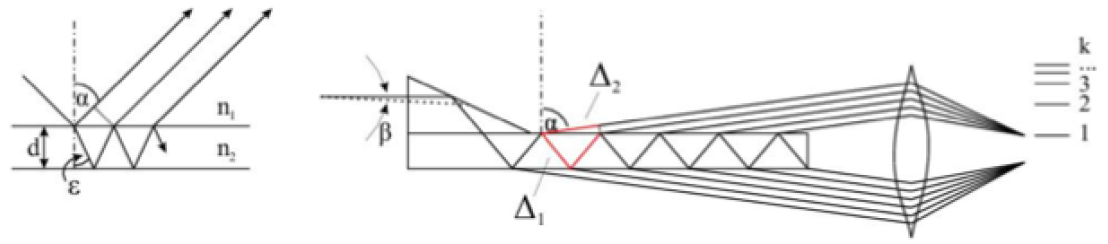
\includegraphics[scale=0.5]{parts/lummerGehrckePlate}
    	\caption{Lummer - Gehrcke - Platte}\label{fig:lummerGehrckePlatte}
    \end{figure}

    In diesem Versuch wird eine Lummer - Gehrcke - Platte verwendet wodurch eine sehr hohe Auflösung erreicht wird, um den Effekt beobachten zu können. Die Platte besteht aus einer Quarzglasplatte mit extremen planparallelen Oberflächen. Das Licht wird durch ein Prisma in die Platte eingekoppelt und danach an den Innenseiten der planparallelen Platten unter einem Winkel nahe der Totalreflexion reflektiert. Die ausfallenden Lichtstrahlen interferieren miteinander und ermöglichen eine sehr hohe Auflösung. Der Gangunterschied ermittelt sich über
    \begin{align}
    	\Delta = 2n_2 \cdot \frac{d}{cos(\epsilon)} - 2n_1 \cdot d \cdot tan(\epsilon) \cdot sin(\alpha)
    \end{align}
    wobei $d$ die Dicke der Platte, $n_1$ und $n_2$ die Brechungsindizes außerhalb und innerhalb der Platte. Die Bezeichnungen $\alpha$ und $\epsilon$ sind aus \autoref{fig:lummerGehrckePlatte} zu entnehmen.

    Aus geometrischen Relationen und der Näherung $n_2 \sim n$, $n_{air} = n_1 \sim 1$ und Austrittswinkel $\alpha \sim 90^\circ$ erhält man
    \begin{align}
    	\Delta = \Delta_1 - \Delta_2 = 2d \cdot \sqrt{n^2 - 1}
    \end{align}
    Für konstruktive Inteferenz muss der Gangunterschied $\Delta = k \cdot \lambda$ mit $k \in \mathbb{N} $ und $\lambda$ die Wellenlänge betragen.

    Den freien Spektralbereich der Lummer - Gehrcke - Platte erhält man über
    \begin{align}
    	\Delta \lambda = \frac{\lambda^2}{2d \cdot \sqrt{n^2 - 1}}
    \end{align}
    Eine kleine Änderung in der Wellenlänge $\delta \lambda << \Delta \lambda$ führt zu einer Verschiebung
    \begin{align}
    	\delta \lambda = \frac{\delta a}{\Delta a} \cdot \Delta \lambda
    \end{align}
    wobei $\delta a$ die Distanz zwischen der Linie mit Wellenlänge $\lambda + \delta \lambda$ und der Position der Linie mit Wellenlänge $\lambda$; $\Delta a$ die Distanz zwischen den zwei Ordnungen $k$ und $k + 1$ der Wellenlänge $\lambda$.

  \subsection{Czerny-Turner Spektrometer}
    \begin{figure}[H]
    	\centering
    	%Quelle von dem Graphen
    	%https://de.wikipedia.org/wiki/Monochromator#/media/File:Czerny-turner.png
    	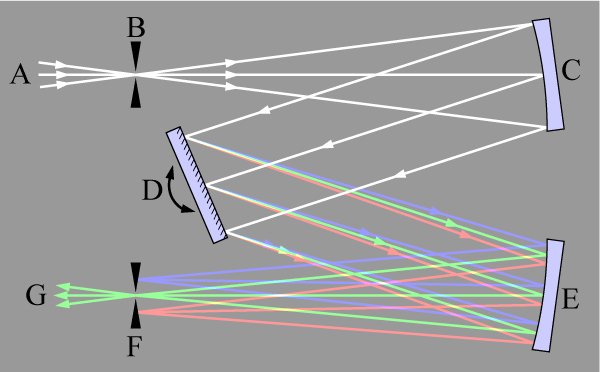
\includegraphics[scale=0.5]{parts/czernyTurnerSpectrometer_Wikipedia}
    	\caption{Czerny - Turner Spektrometer}\label{fig:czernyTurnerSpectrometer}
    \end{figure}

    Licht, welches in das Spektrometer eintritt, wird zuerst mit Hilfe eines konkaven Spiegels parallelisiert. Danach trifft es auf ein Gitter und wird gebrochen. Das gebrochene Licht wird über einen weiteren konkaven Spiegel fokusiert und trifft anschließend auf eine CCD Kamera (siehe \autoref{fig:czernyTurnerSpectrometer}).

    Die Dispersionseigenschaften eines Spektrokopieelements kann über eine Funktion $D(\lambda)$, bezogen auf wechselwirkende lineare Dispersion, beschrieben werden
    \begin{align}
    	D(\lambda) = \frac{\delta \lambda}{\delta p}
    \end{align}
    wobei $p$ die Position (bei der CCD Kamera in Pixel). Somit kann die Wellenlänge als Funktion der Position ermittelt werden
    \begin{align}
    	\lambda = \lambda_0 + \int_{p_0}^{p} D(\lambda) \; dp \label{lambdadispersion}
    \end{align}
    wobei $\lambda_0$ und $p_0$ bekannte Referenzpunkte sind. Ist die Dispersionsrelation unabhängig von $\lambda$ so kann Gleichung \eqref{lambdadispersion} vereinfacht werden zu
    \begin{align}
    	\lambda = \lambda_0 + D(p - p_0)
    \end{align}

    \begin{figure}[H]
    	\centering
    	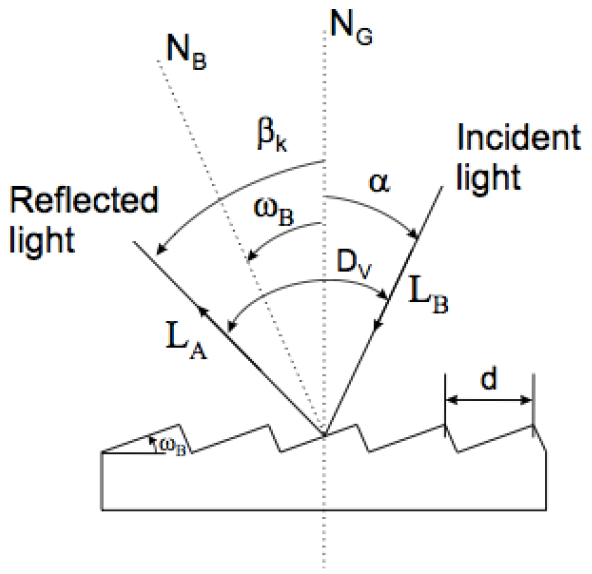
\includegraphics[scale=0.5]{parts/schematicReflectionGrating}
    	\caption{Schematische Darstellung einer Gitterreflexion}\label{fig:schematicReflexionGrating}
    \end{figure}

  \section{Teil 1: Bohr'sches Magneton}
  \subsection{Hysterese-Effekt}
    Mit dem Teslameter wird die Stärke des Magnetfeldes zwichen den Spulen bei 6 Stromstärken, von \SI{8}{\ampere} bis \SI{13}{\ampere}, gemessen. Für den Fehler nehmen wir \SI{0.1}{\ampere} an. Der Hysterese-Effekt wird nun eingeschätzt, indem wir den Zusammenhang zwischen Stromstärke und Magnetfeld ermitteln. Und wir führen diese Messung sowohl bei fallender als auch bei steigender Stromstärke durch. Für alle Messpunkte gilt: wir nutzen drei Messwerte und bilden daraus ein Mittel. (s. \hyperref[plot::1]{Abb. \ref*{plot::1}})\\\\
    Die aus den Werten ermittelten linearen Fits ergaben folgende Steigungen:\\\\
    \textbf{bei aufsteigender Stromstärke:}
      \begin{align}
        m_u = \SI{39.461+-2.198}{\milli\tesla\per\ampere}
      \end{align}
    \textbf{bei absteigender Stromstärke:}
      \begin{align}
        m_d = \SI{38.874+-2.192}{\milli\tesla\per\ampere}
      \end{align}\\
    Die beiden Geraden stimmen dabei mit weniger als \SI{1}{\sigma} überein, und in unserem Fall kann der Hsyterese-Effekt vernachlässigt werden. Für die folgenden Berechnungen wird ein Mittel gebildet, es ergibt sich für den Zusammenhang zwischen Strom und Magnetfeld:
    \begin{align}
      B(I) = \SI{39.168+-1.552}{\milli\tesla\per\ampere} \cdot I + \SI{130.765+-15.849}{\milli\tesla}
    \end{align}
    (Die Fehler erhält man mittels Fehlerfortpflanzung)

    \begin{figure}[H]
      \centering
      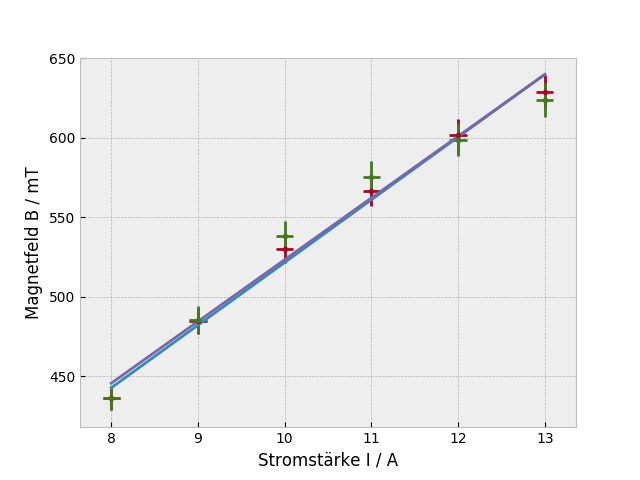
\includegraphics[width=.6\paperwidth]{Auswertung/hysteresis}
      \caption{Hysterese}
      \label{plot::1}
    \end{figure}

  \subsection{Polarisation}
    Das Licht der Cadmium Lampe wird in longitudinaler und transversaler Richtung zum Magnetfeld beobachtet. Durch Verwendung eines linearen Polarisationsfilters und eine $\lambda$/4-Plättchens kann die Polarisation analysiert werden.

    \subsubsection{Beobachtung in longitudinaler Richtung}
      Bei dieser Beobachtungsrichtung sind sowohl mit als auch ohne linearen Polarisationsfilter zwei Linien pro Beugungsordnung zu sehen. Daraus ist zu schließen, dass es sich bei dem Licht um zirkular polarisiertes Licht handelt. (s. \hyperref[pic::1]{Abb. \ref*{pic::1}})

      Wandelt man nun mit Hilfe des $\lambda$/4-Filters das Licht in linear polarisiertes um, so kann man mit dem Polarisationsfilter eine der beiden Linien herausfiltern und bei Rotation um \SI{90}{°} des $\lambda$/4-Filters die jeweils andere beobachten. (s. \hyperref[pic::2]{Abb. \ref*{pic::2}})

      \begin{figure}[H]
        \centering
        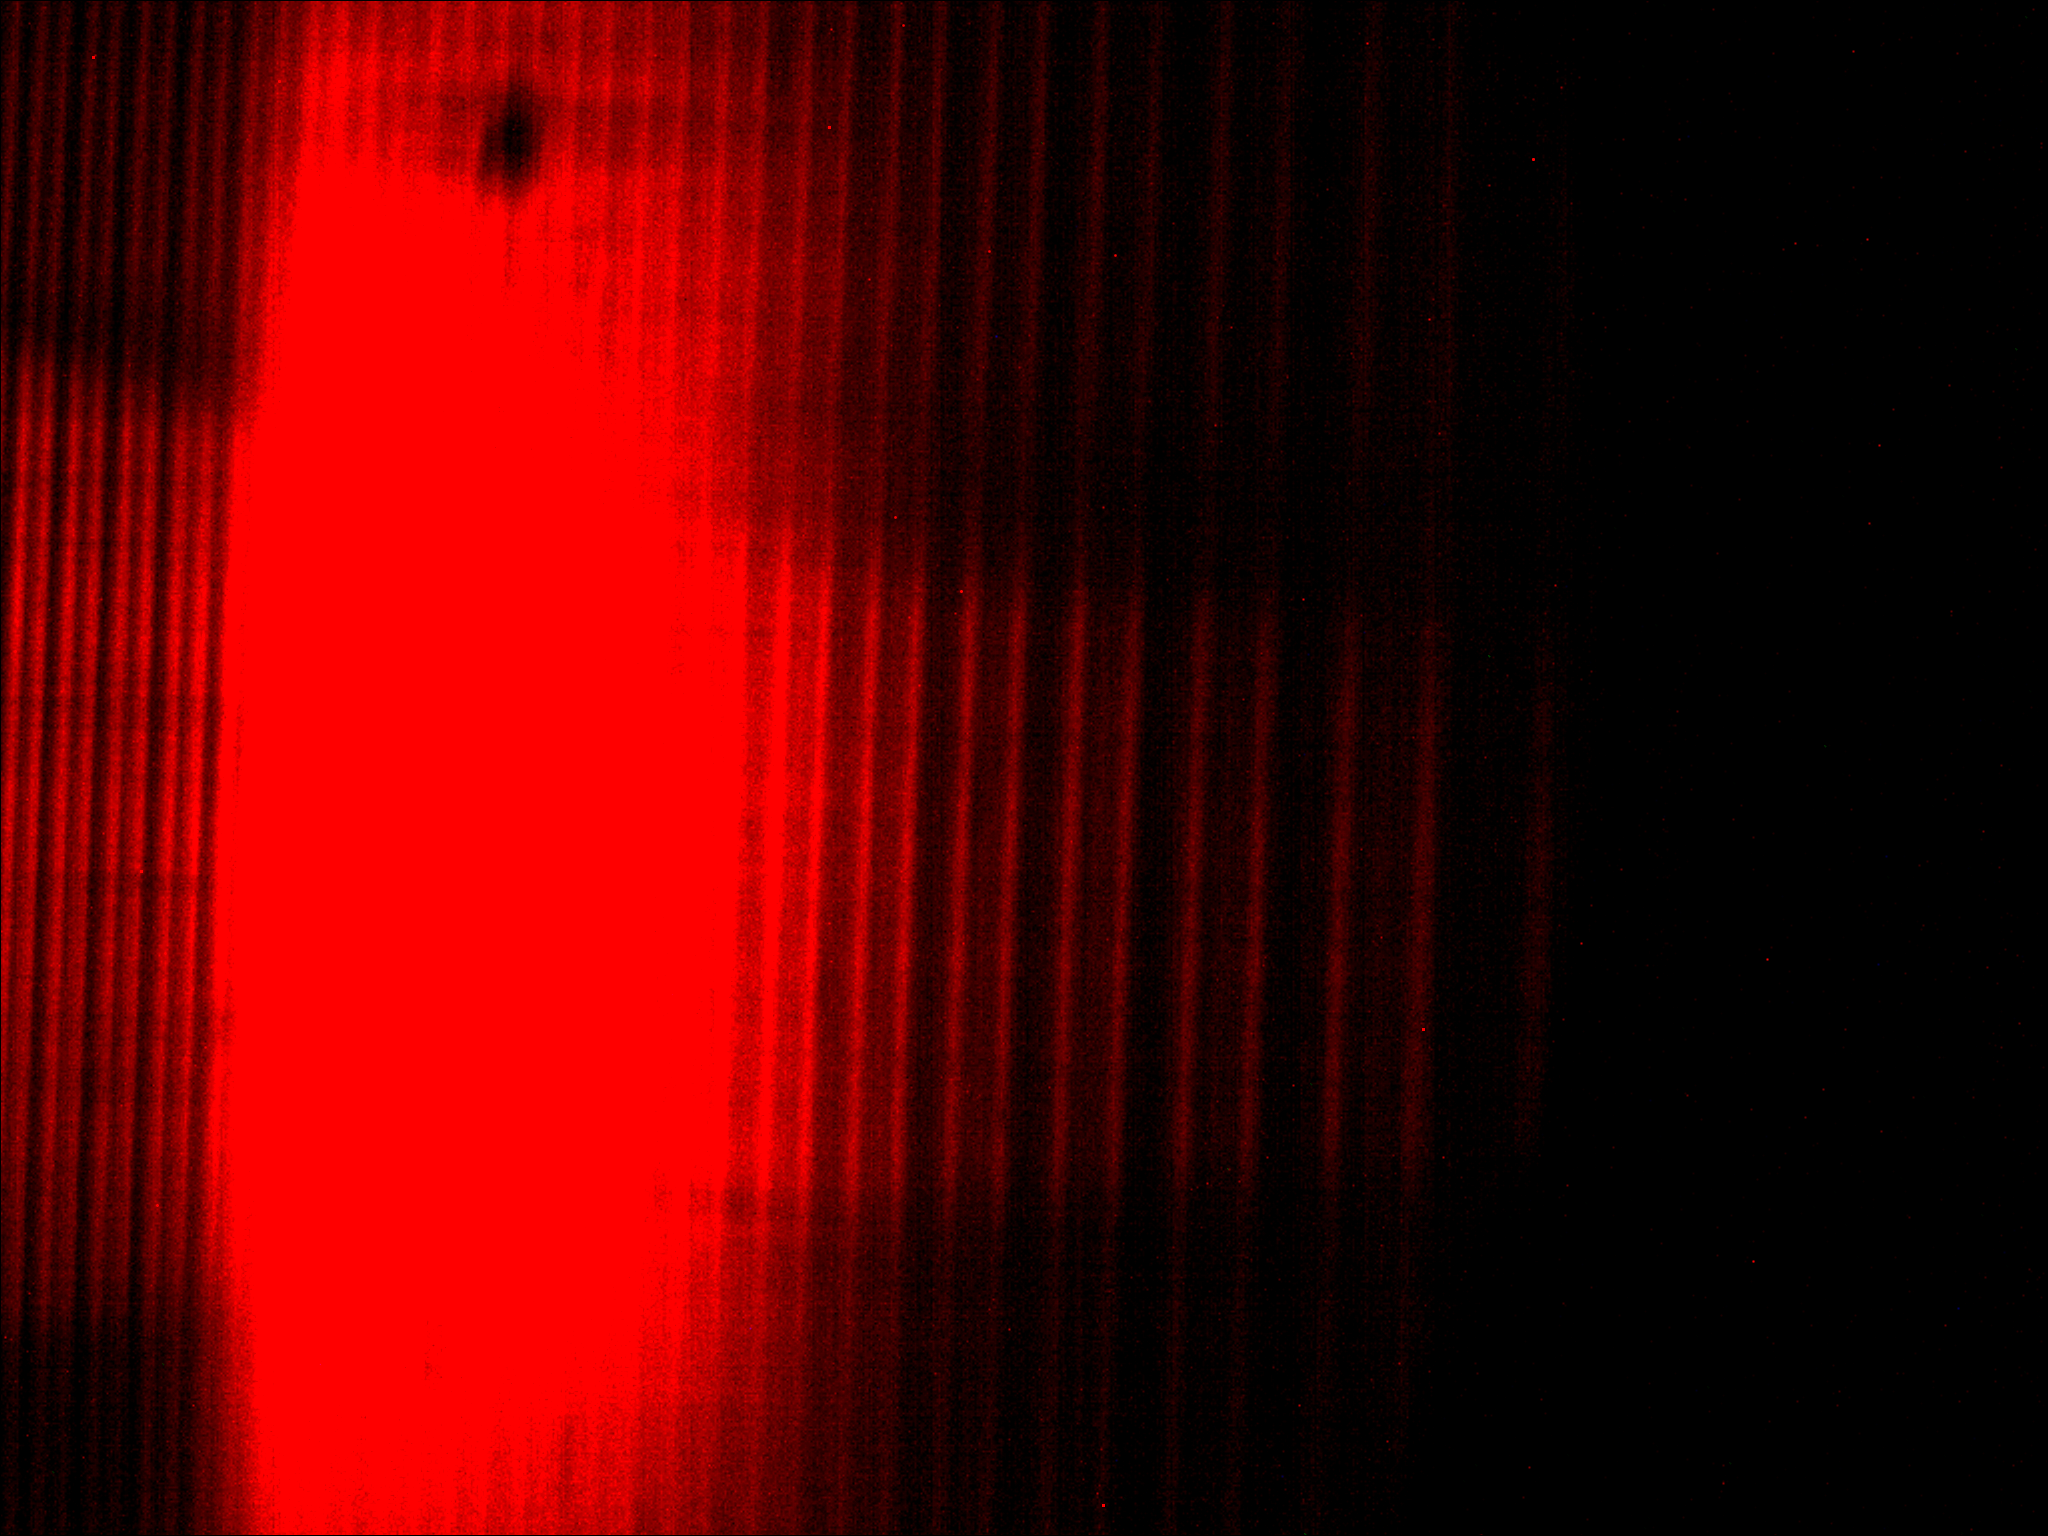
\includegraphics[width=.6\paperwidth, trim={0 200pt 0 400pt}, clip]{Auswertung/data/long/10A_0}
        \caption{Beobachtete Linien in longitudinaler Ausrichtung, ohne Filter}
        \label{pic::1}
      \end{figure}
      \begin{figure}[H]
        \centering
        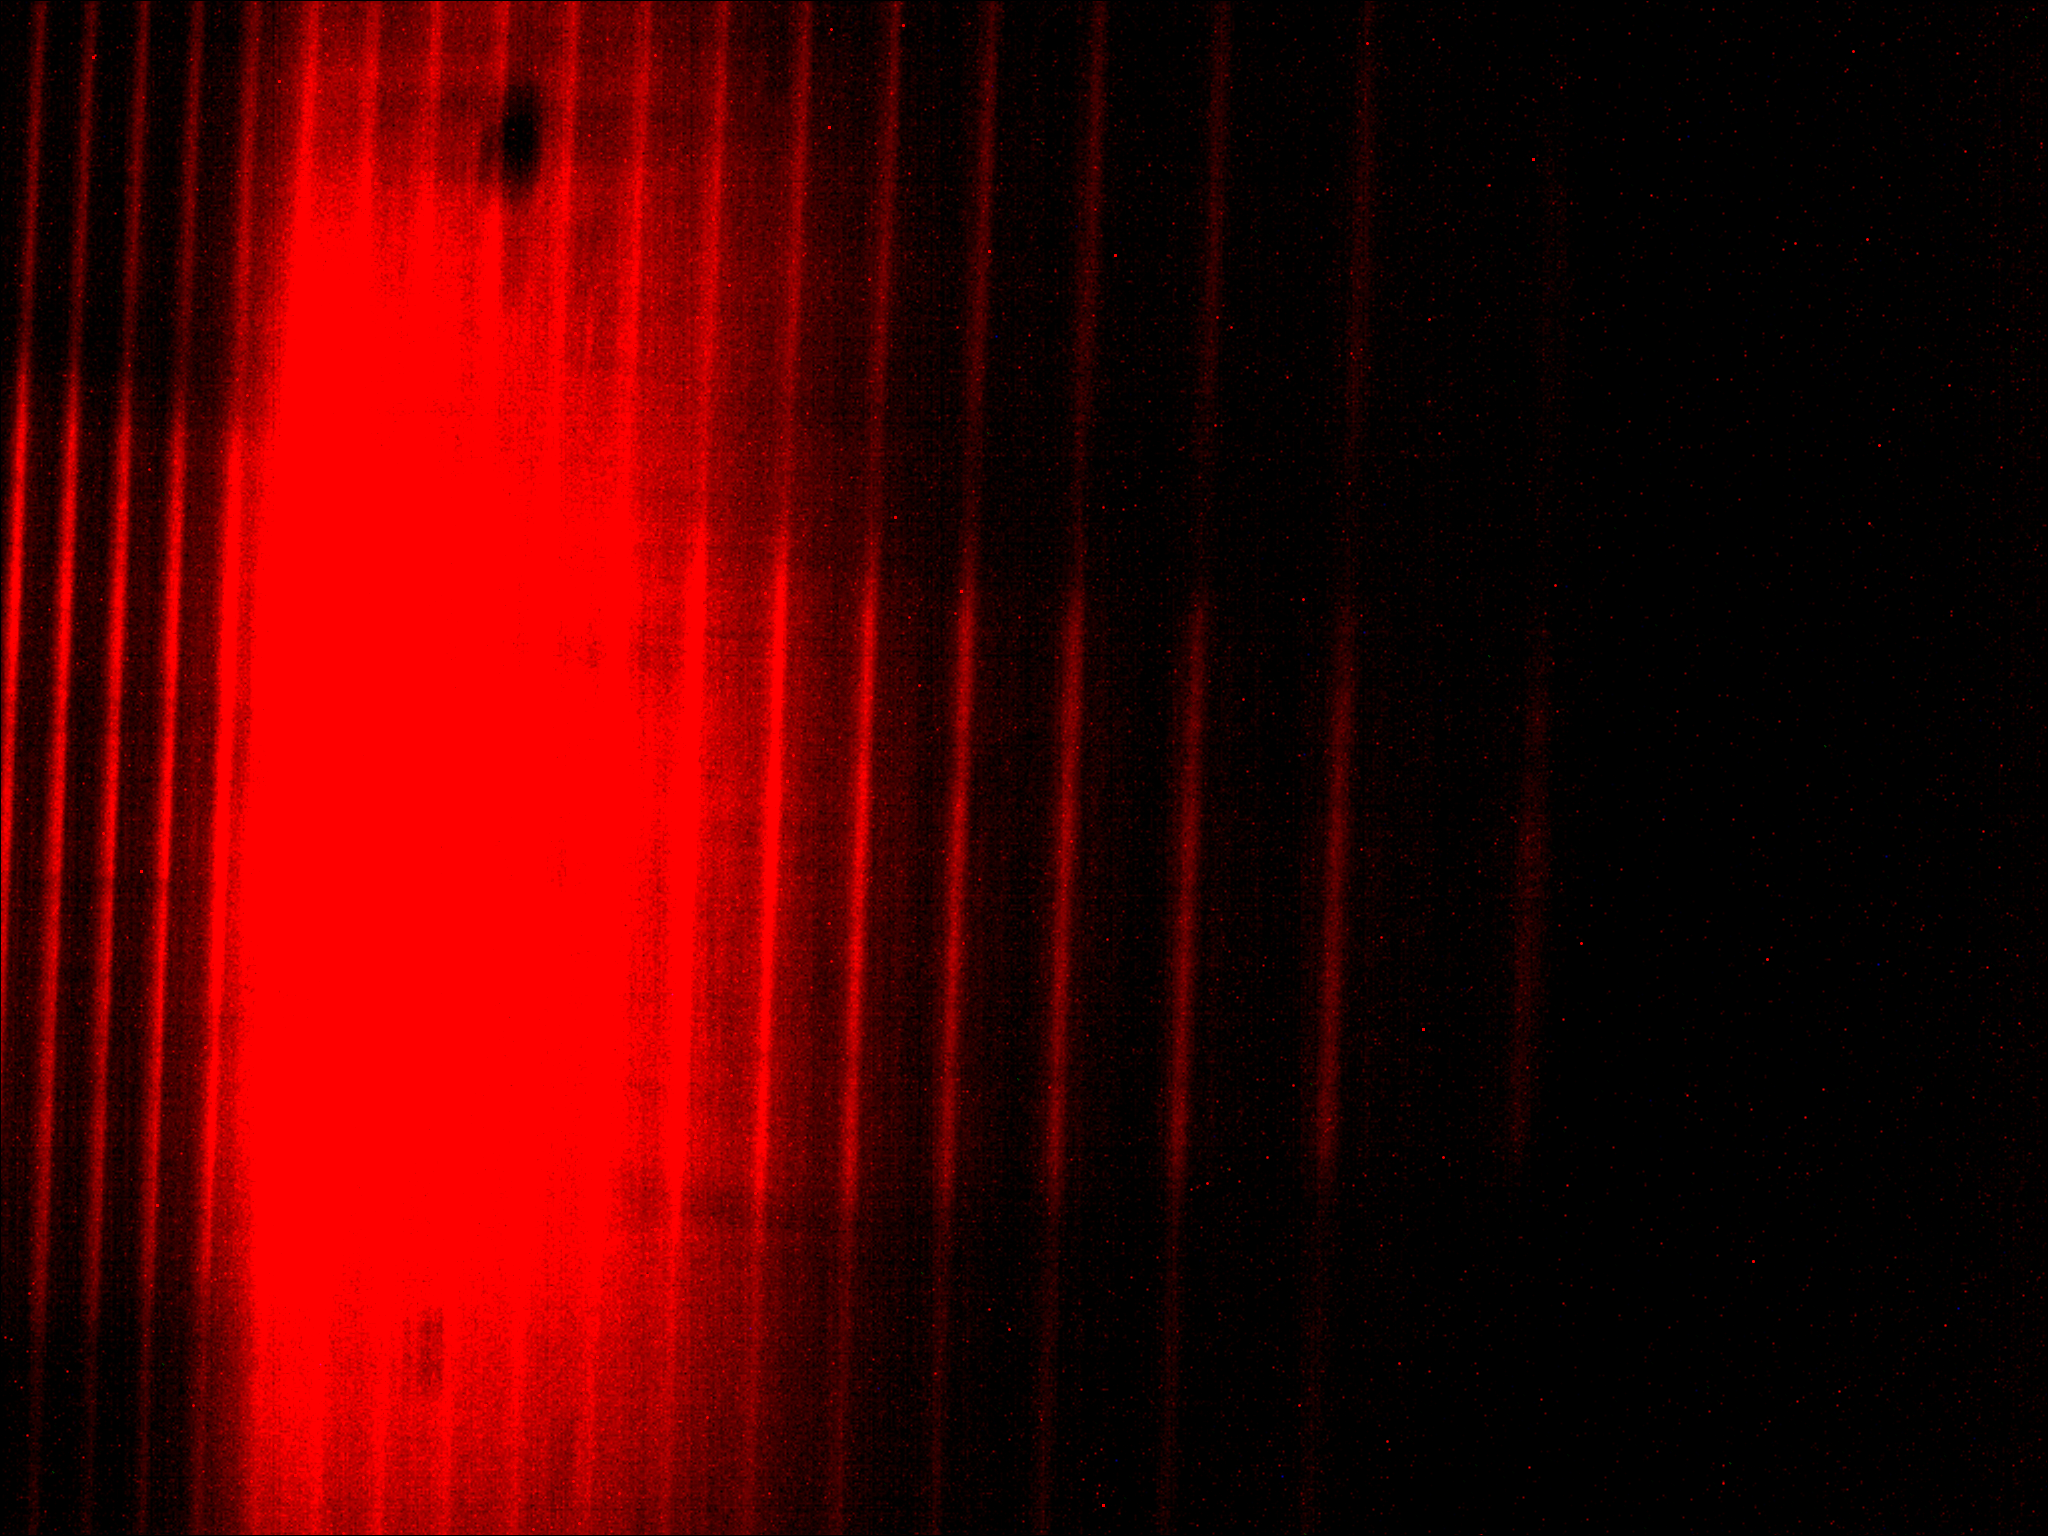
\includegraphics[width=.6\paperwidth, trim={0 650pt 0 200pt}, clip]{Auswertung/data/long/10A_2}
        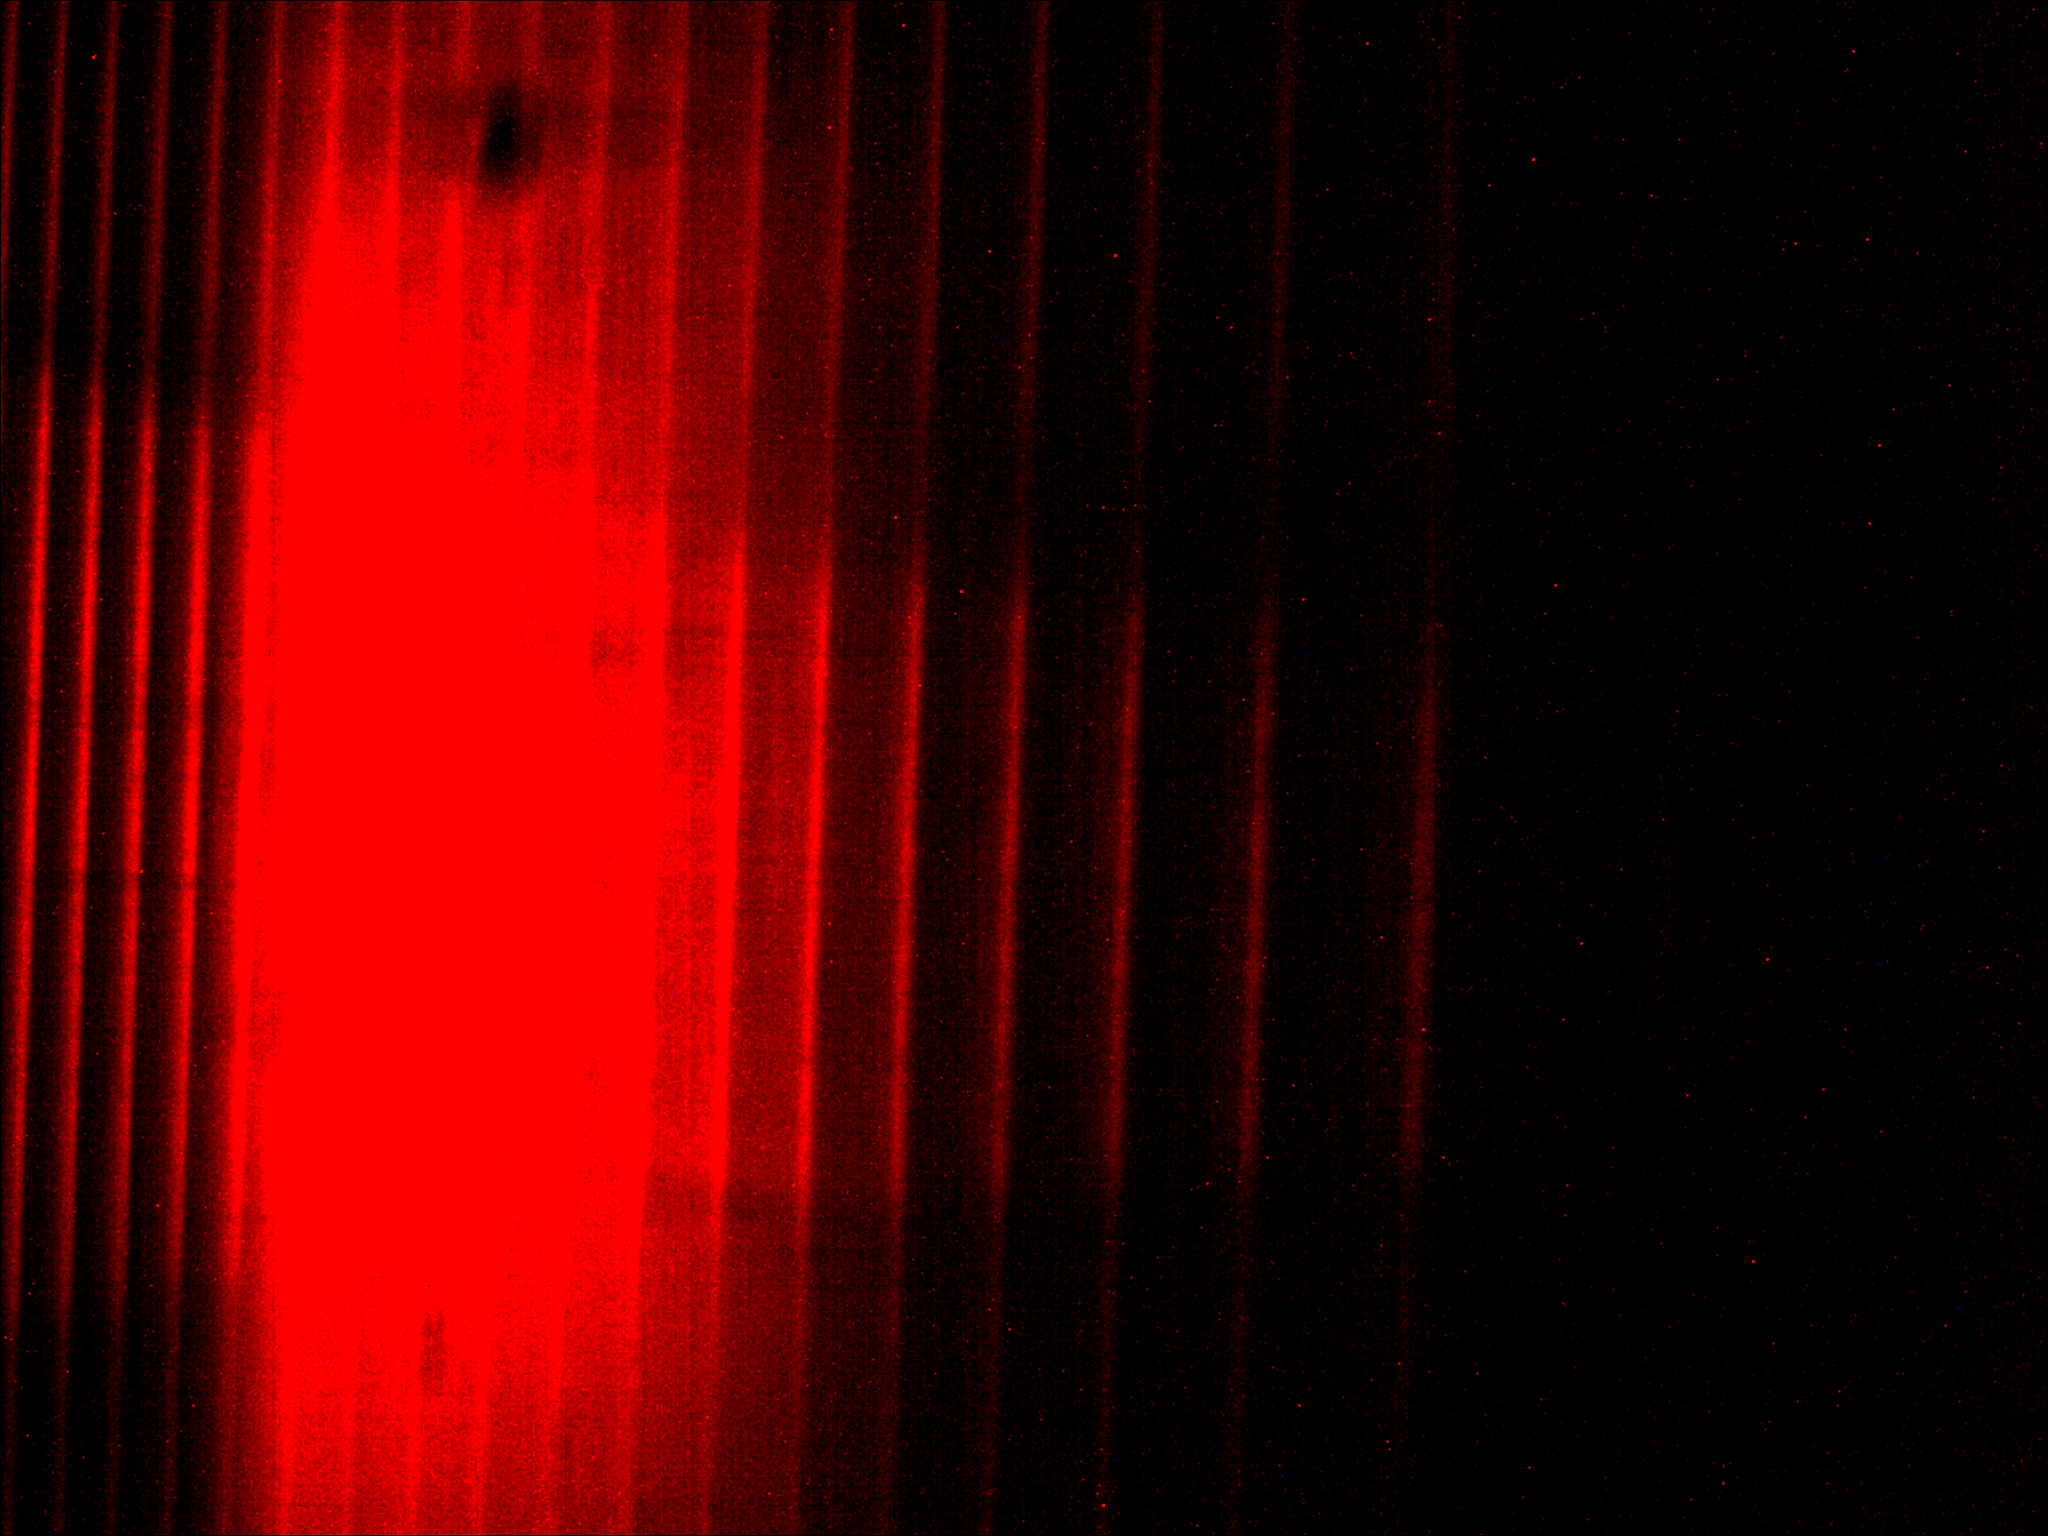
\includegraphics[width=.6\paperwidth, trim={0 0 0 886pt}, clip]{Auswertung/data/long/10A_1}
        \caption{Beobachtete Linien in longitudinaler Richtung, mit $\lambda$/4-Filter und linearem Polarisationsfilter}
        \label{pic::2}
      \end{figure}
    \newpage
    \subsubsection{Beobachtung in transversaler Richtung}
      Hier können wir eine Aufspaltung in drei Linien beobachten. Der Polarisationsfilter lässt entweder die beiden äusseren Linen ($\sigma$-Linien) verschwinden, oder nach einer \SI{90}{\deg} Drehung die mittlere Linie ($\pi$-Linie) (s. \hyperref[pic::3]{Abb. \ref*{pic::3}}). Das Licht ist also linear polarisiert, mit senkrechter Polarisationsrichtung zwichen $\sigma$- und $\pi$-Linien

      \begin{figure}[H]
        \centering
        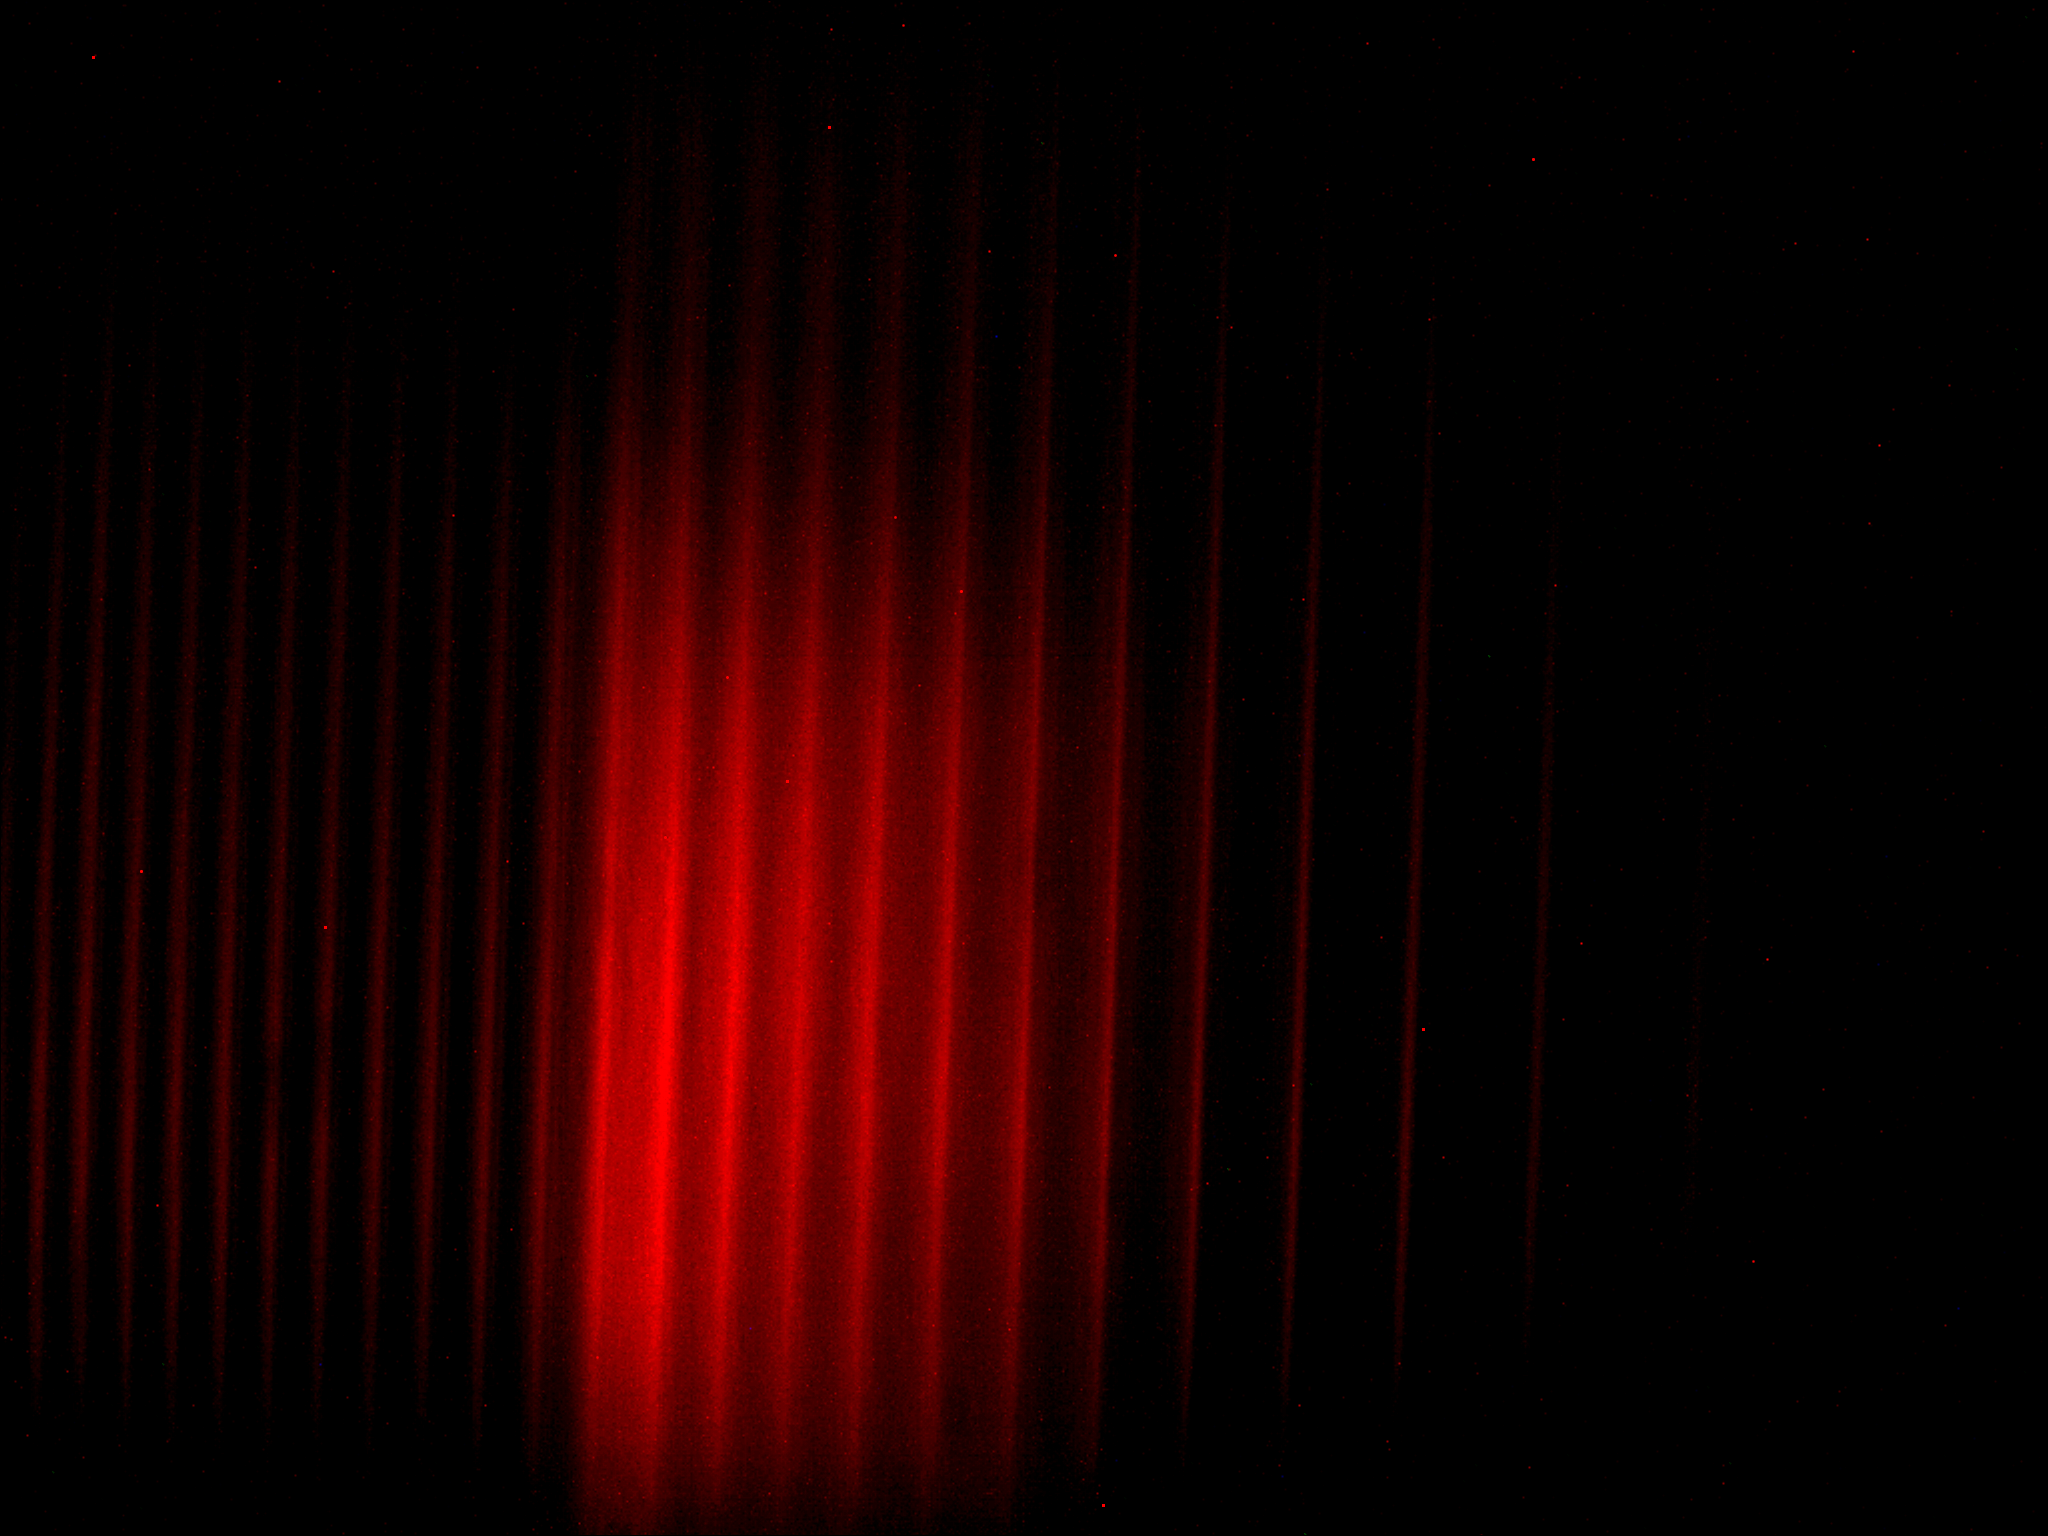
\includegraphics[width=.6\paperwidth, trim={0 300pt 0 900pt}, clip]{Auswertung/data/trans/10A/10A_pi}
        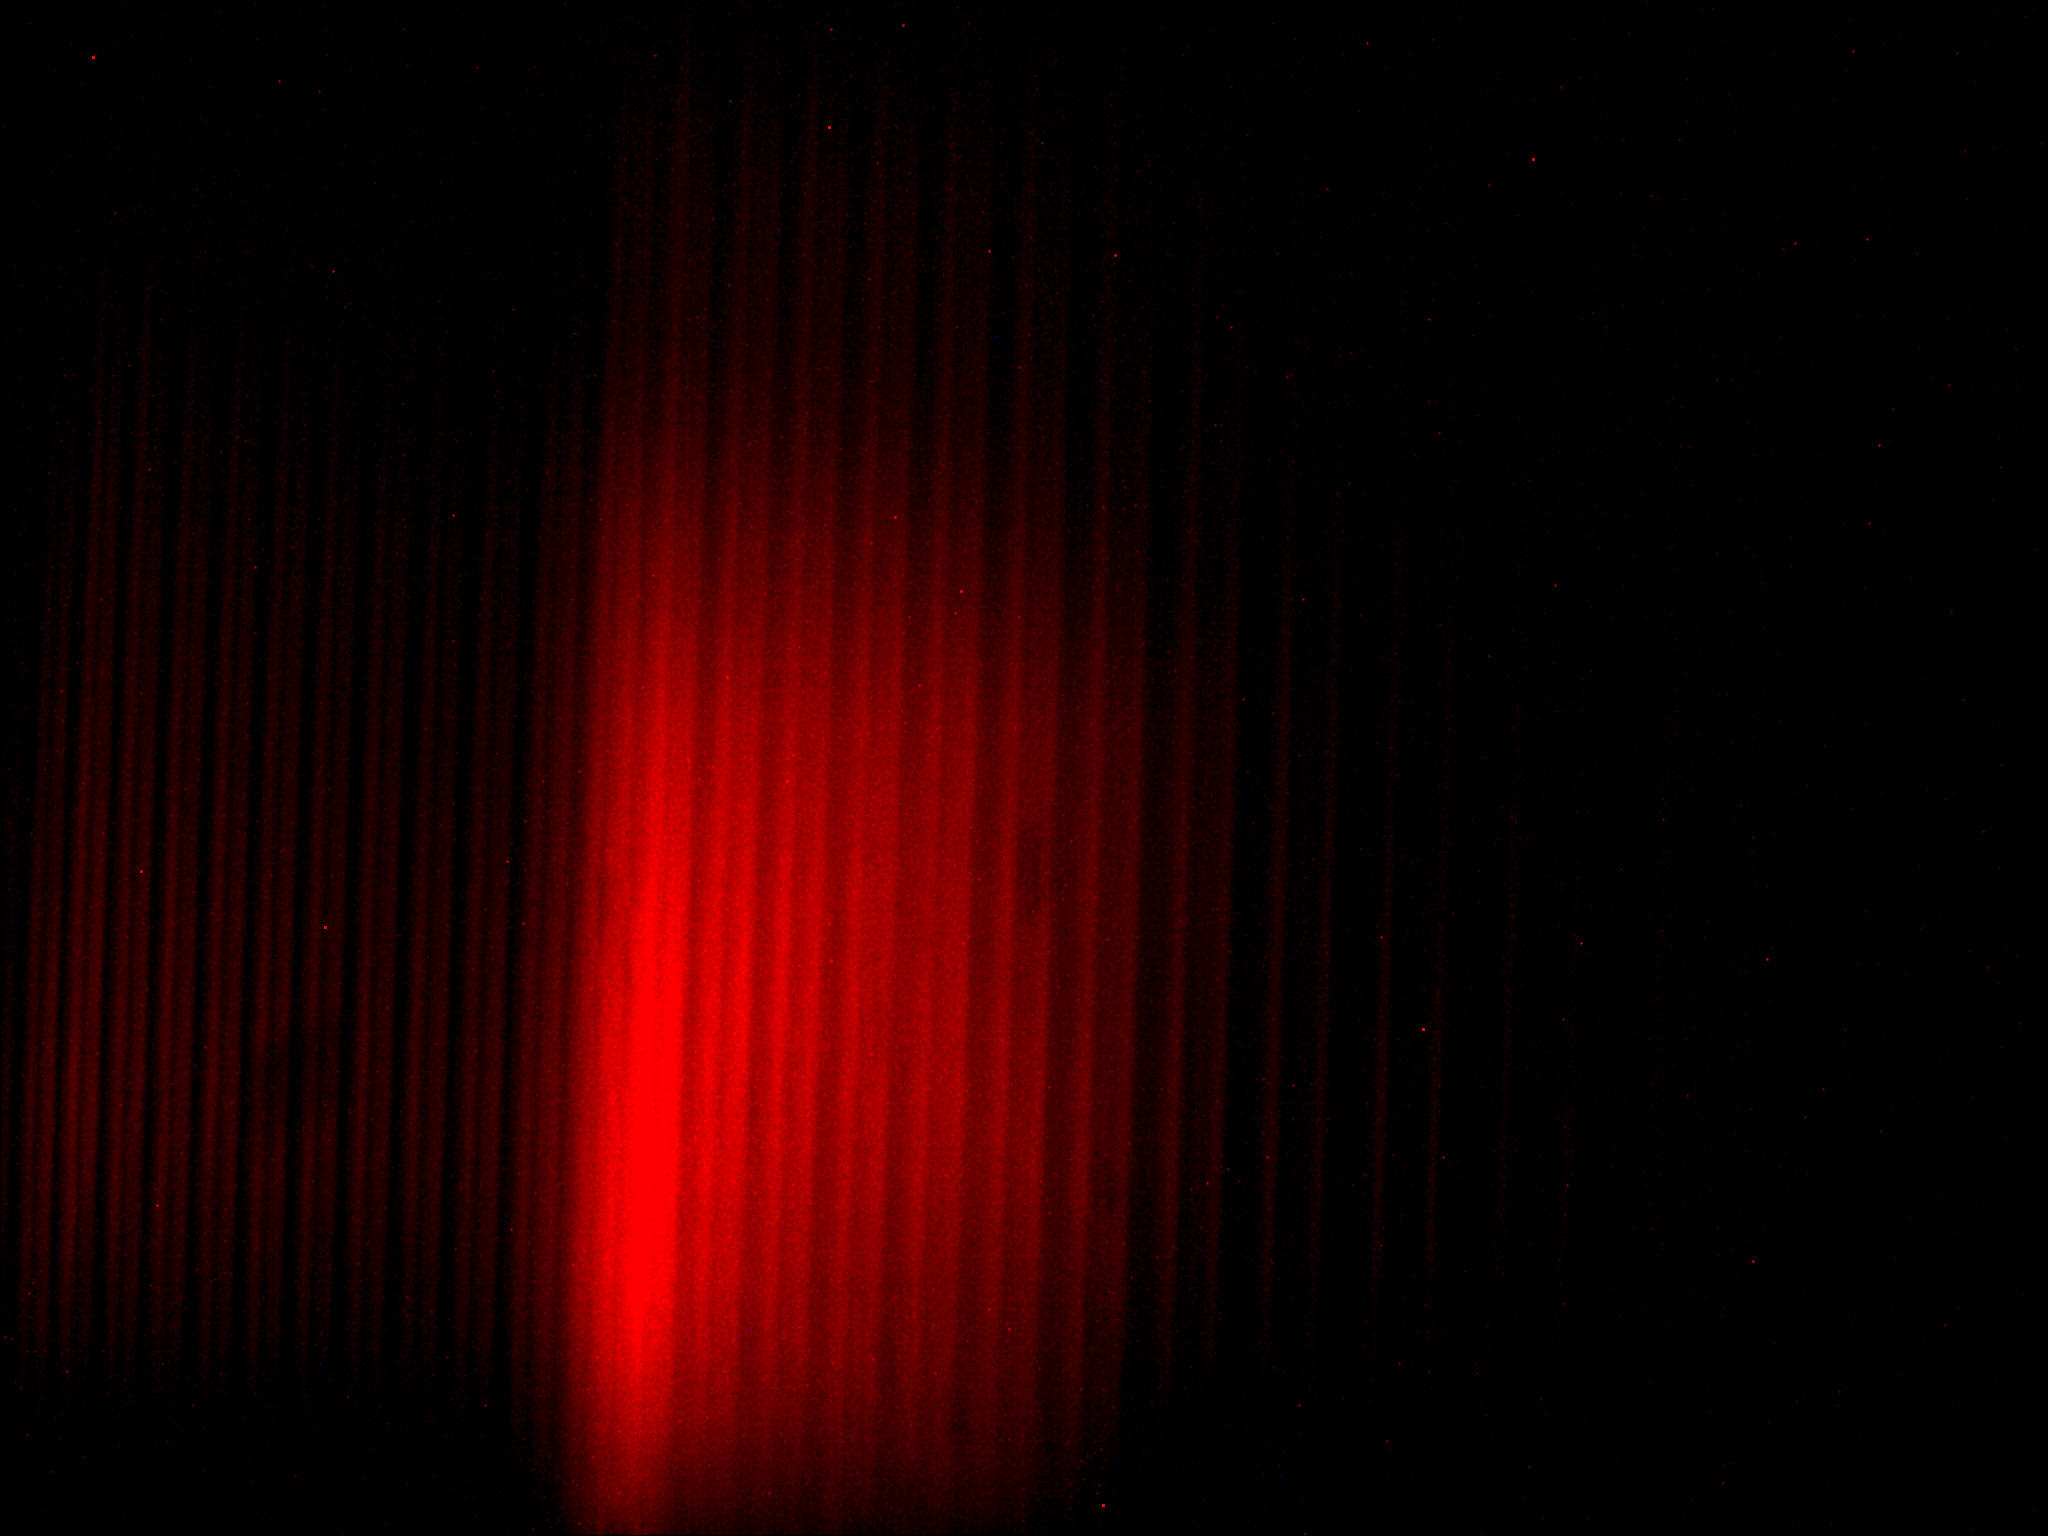
\includegraphics[width=.6\paperwidth, trim={0 300pt 0 900pt}, clip]{Auswertung/data/trans/10A/10A_sig}
        \caption{Beobachtete Linien in transversaler Ausrichtung, mit linearem Polarisationsfilter}
        \label{pic::3}
      \end{figure}

      Bei Variation der Stromstärke und des damit resultierenden Magnetfeldes, kann man beobachten, dass die Aufspaltung der Spektrallinien mit zunehmender Stromstärke größer wird.

      \begin{figure}[H]
        \centering
        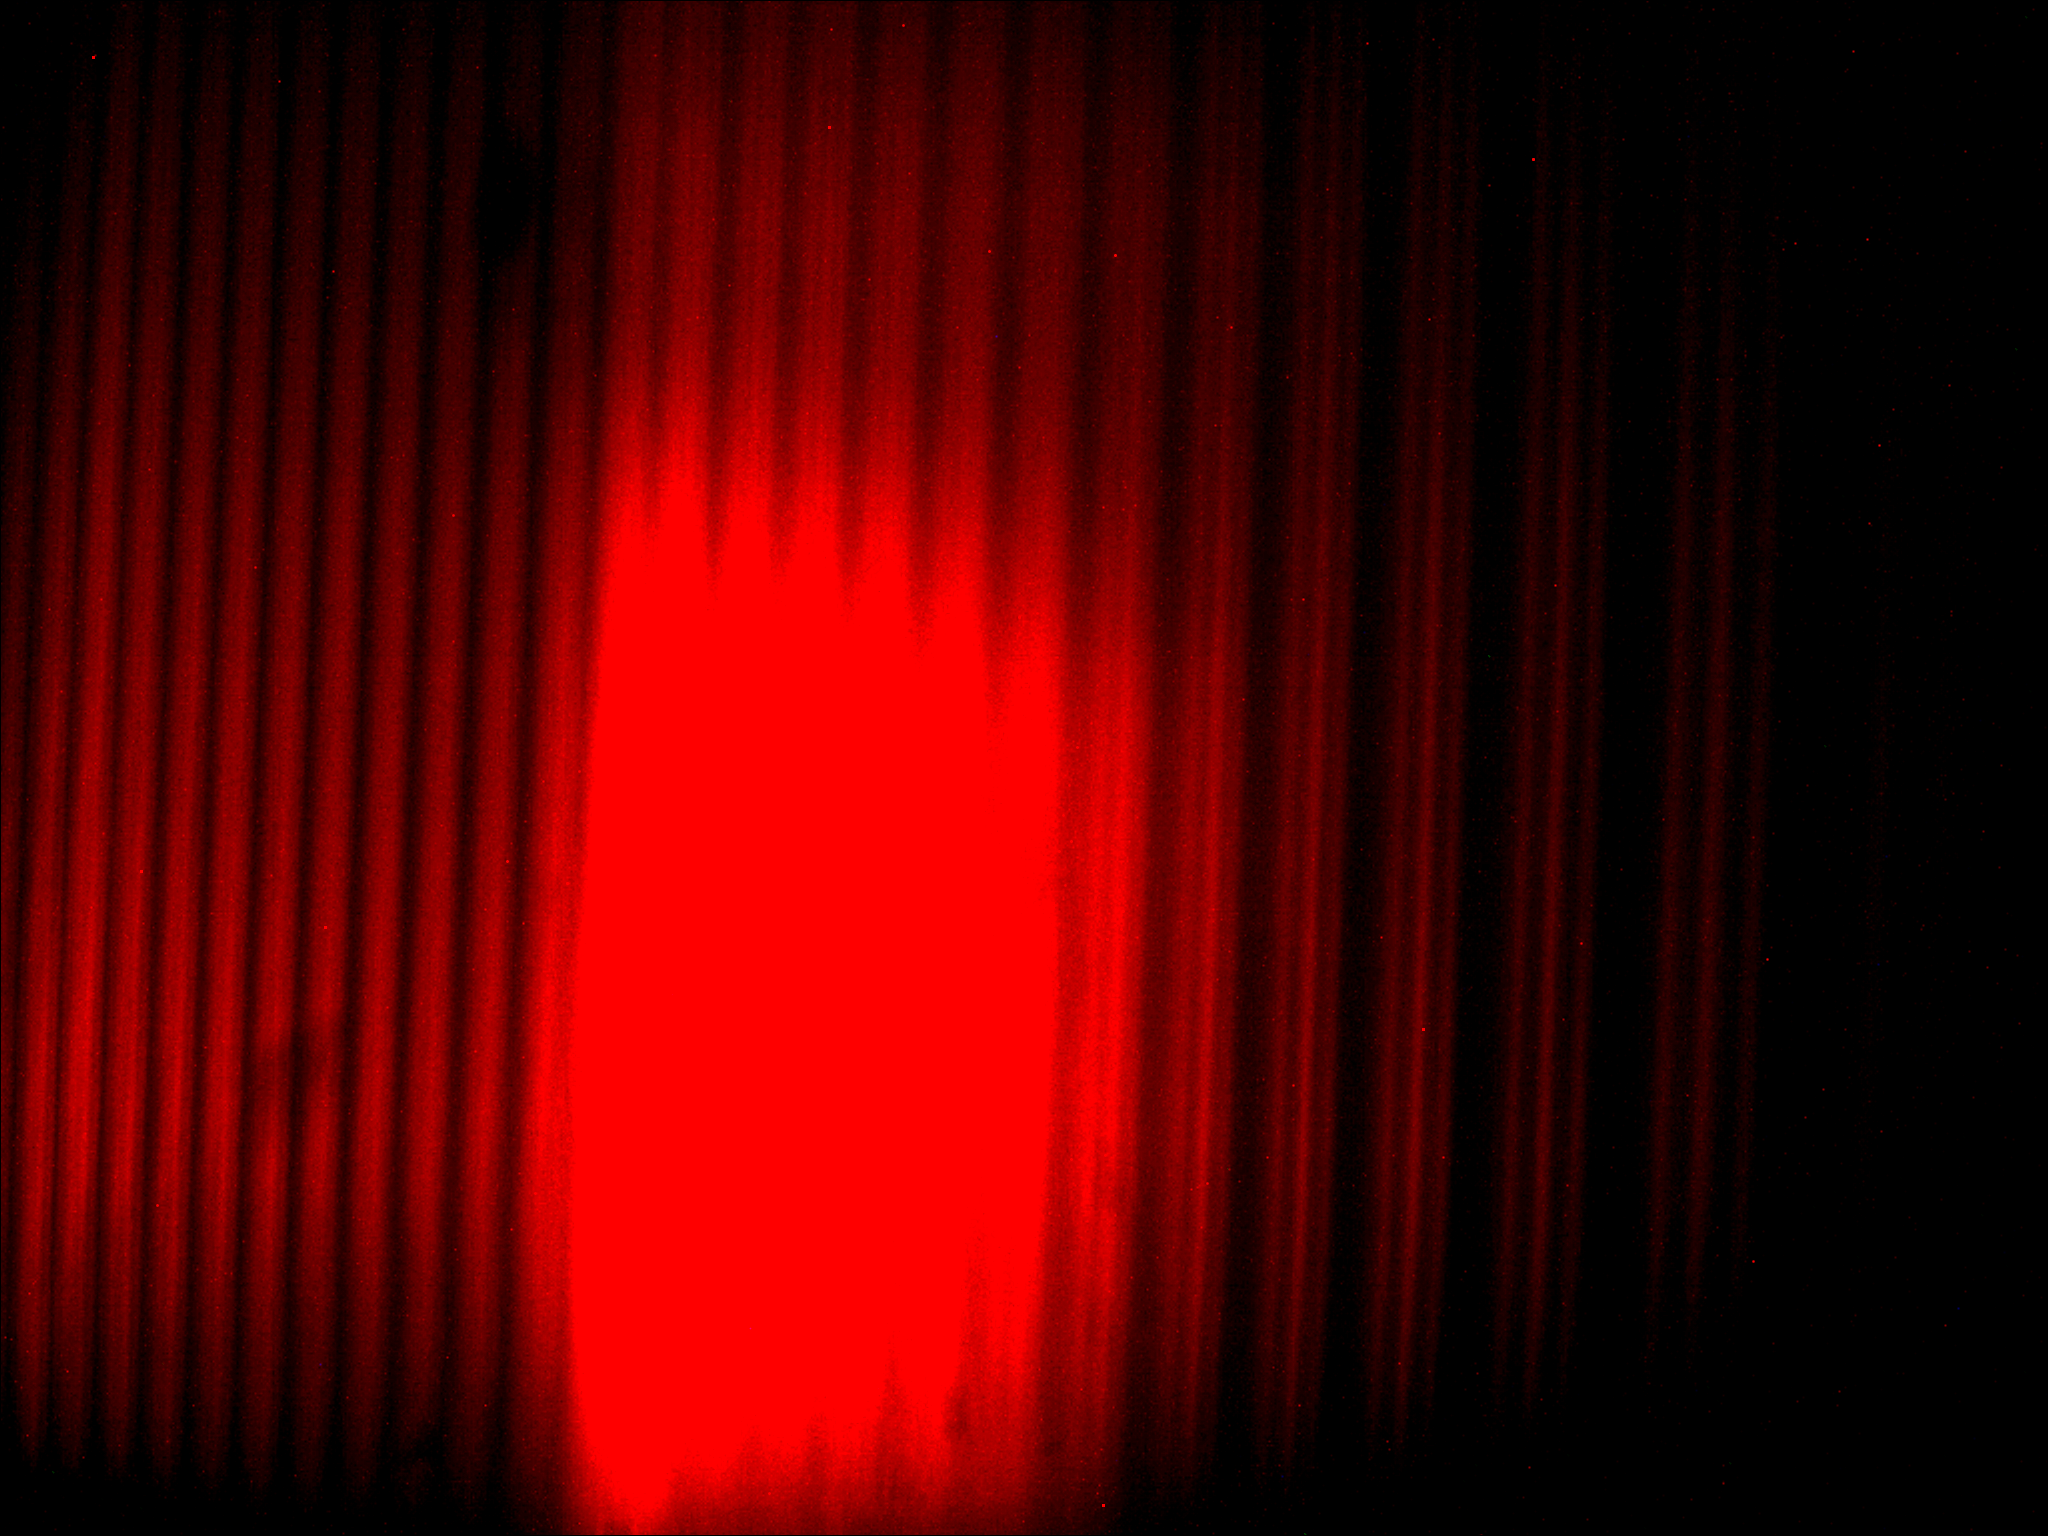
\includegraphics[width=.6\paperwidth,trim={0 600pt 0 500pt}, clip]{Auswertung/data/trans/10A/10A_l}
        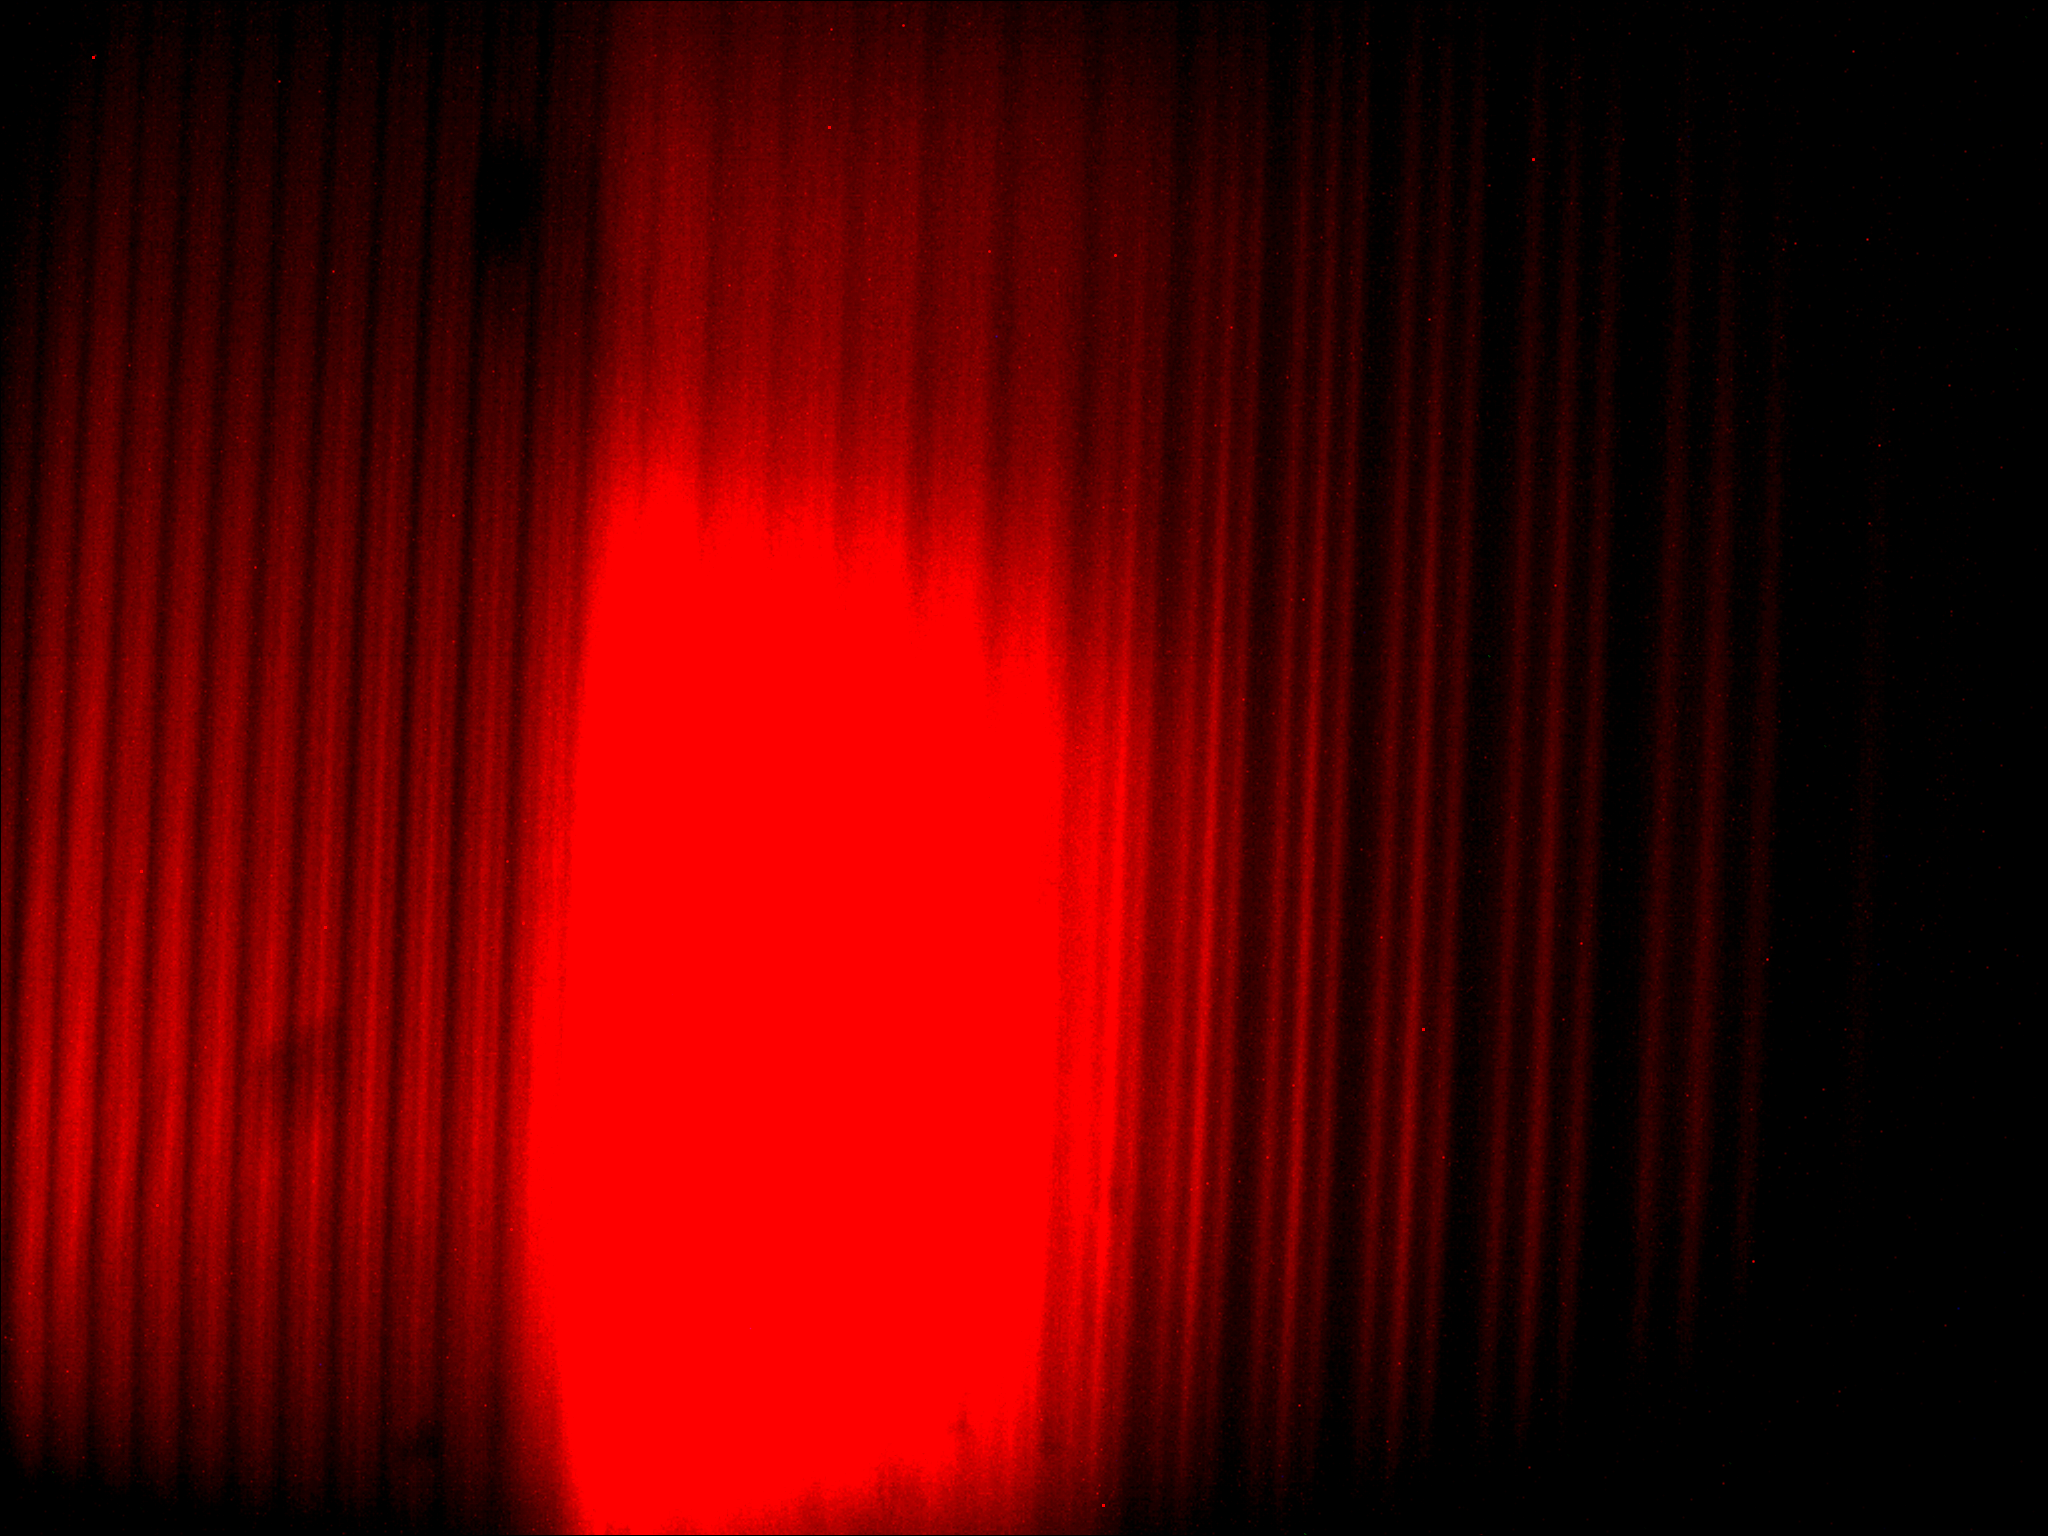
\includegraphics[width=.6\paperwidth,trim={0 200pt 0 900pt}, clip]{Auswertung/data/trans/13A/13A_l}
        \caption{Beobachtete Linien in transversaler Richtung, bei 10A (oben) und 13A (unten)}
        \label{pic::4}
      \end{figure}

    \subsection{Bestimmung der Wellenlängenverschiebung}
      \subsubsection{Position der $\pi$- und $\sigma$-Linien}
        Wir nutzen das Programm \textbf{JImage} um die zweidimensionalen Bilder, der beobachteten spektralen Aufspaltung in eine eindimensionale Intensitätsverteilung zu konvertieren. Mit \textbf{Python}\footnote{Repo mit den benutzten Skripten zur Auswertung:  \href{github.com/acereca/FP/tree/master/F44 - Zeemanspektroskopie}{github.com/acereca/FP $\rightarrow$ F44}} kann jetzt die Position (in Pixel) jeder $\pi$- und $\sigma$-Linie von etwa fünf Ordnungen (wegen der Reflektion in der Mitte der Bilder) pro Messung bestimmt werden.

        Jeder gemessene Peak wird jetzt mit einer Gausskurve gefittet und daraus die Breite und Position bestimmt. Die Gaussfunktion berücksichtigt, dass durch die thermische Bewegung der Atome ein Doppler-Effekt entsteht und dadurch ist die ausgesandte Wellenlänge je nach Bewegungsrichtung des Atoms leicht verschoben, sodass die Linien im Vergleich zur Lorentz-Kurve breiter erscheinen. Als Fehler der Position wird hier der $\sigma^2$-Parameter der Gaussfunktion genutzt
        \begin{align}
          \Delta x = \sigma \cdot 2.4 / 2
        \end{align}
        also die halbe Halbwertsbreite (HWHM).

      \subsubsection{Verschiebung der Ordungen}
        Wir ordnen nun den $\pi$-Linien Ordnungszahlen zu, diese sollten nur diskrete, ganzzahlige Werte sein, allerdings möchten wir den $\sigma$-Linien auch eine solche Ordnung zuordnen, also betrachten wir eine kontinuierliche Fitfunktion. In unserem Fall ist diese eine Polynomfunktion 2. Grades (s. \hyperref[plot::2]{Abb. \ref*{plot::2}}). Diese Beobachtung ist innerhalb unserer Näherung ausreichend, da ein Polynom höheren Grades keine signifikante Verbesserung der Beschreibung unserer Daten liefert.

        Um die Fehler der Beugungsordnung zu bestimmen nutzen wir:
        \begin{align}
          \Delta k(a) = k(a+\Delta a) - k(a)
        \end{align}
        wobei die Fehler der Fitparameter vernachlässigt werden. $a$ ist hier die Position der Linien in Pixel, $k$ die zugeordnete Beugungsordnung.

        Jetzt werden die Verschiebungen der $\sigma$-Linien zur zugehörigen $\pi$-Linie, in Bruchteilen einer Beugungsordnung, berechnet und geplottet (\hyperref[plot::3]{Abb. \ref*{plot::3}}), für die Berechnung dient:
        \begin{align}
          \delta k = k(a) - k_{theo}\\
          \Delta (\delta k) = \Delta k(a)
        \end{align}
        Dabei entspricht die theoretische Beugungsordnung $k_{theo}$ den diskreten Werten, die den $\pi$-Linien zugeornet werden können. Der Fehler geht hier aus dem Fehler der errechneten Beugungsordung der $\sigma$-Linien hervor, da $k_{theo}$ keinen Fehler besitzt.

        \begin{landscape}
          \thispagestyle{empty}
          \begin{figure}
            \vspace*{-2cm}
            \caption{Gefittete Positionen der Peaks}
            \label{plot::2}
            \hspace*{-6cm}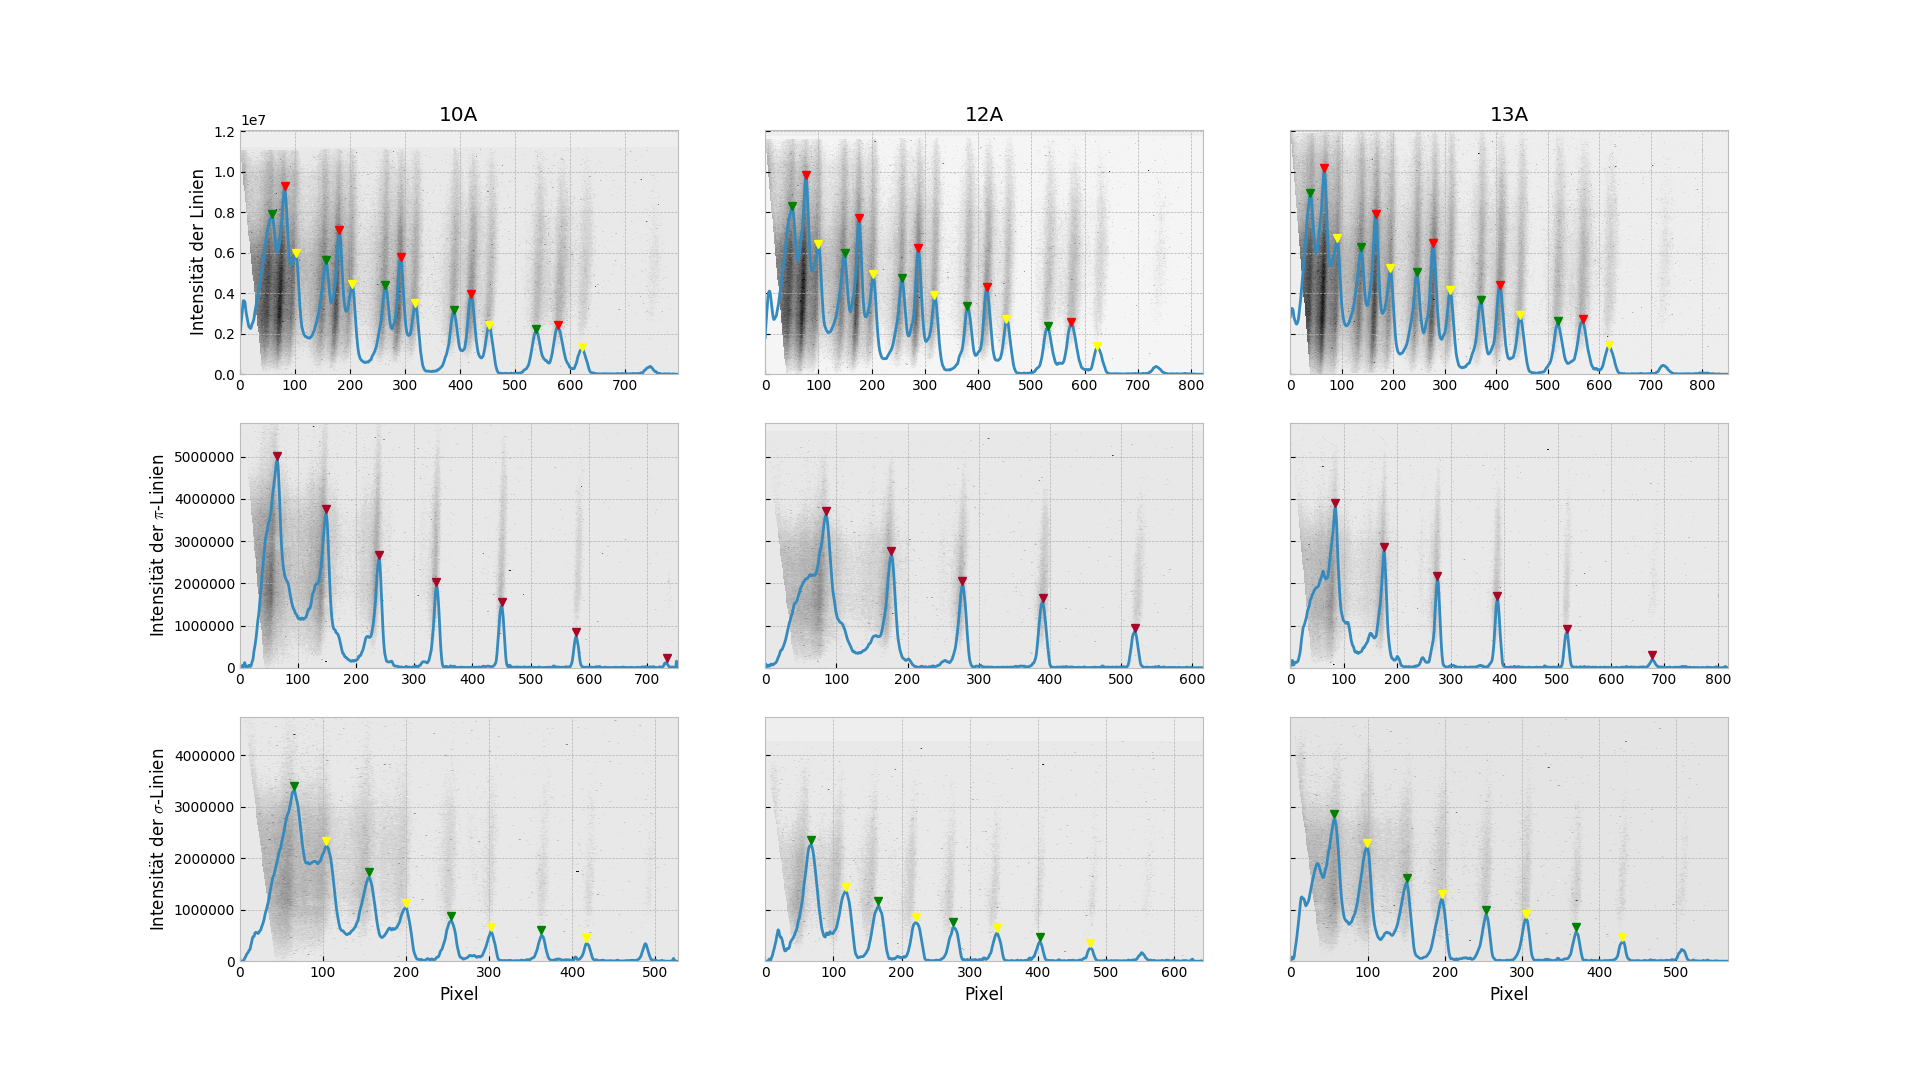
\includegraphics[width=1.5\paperwidth]{Auswertung/peaks}
          \end{figure}
        \end{landscape}
        \begin{landscape}
          \thispagestyle{empty}
          \begin{figure}
            \vspace*{-2cm}
            \caption{Polynomfits für die drei Stromstärken}
            \label{plot::3}
            \hspace*{-5cm}
            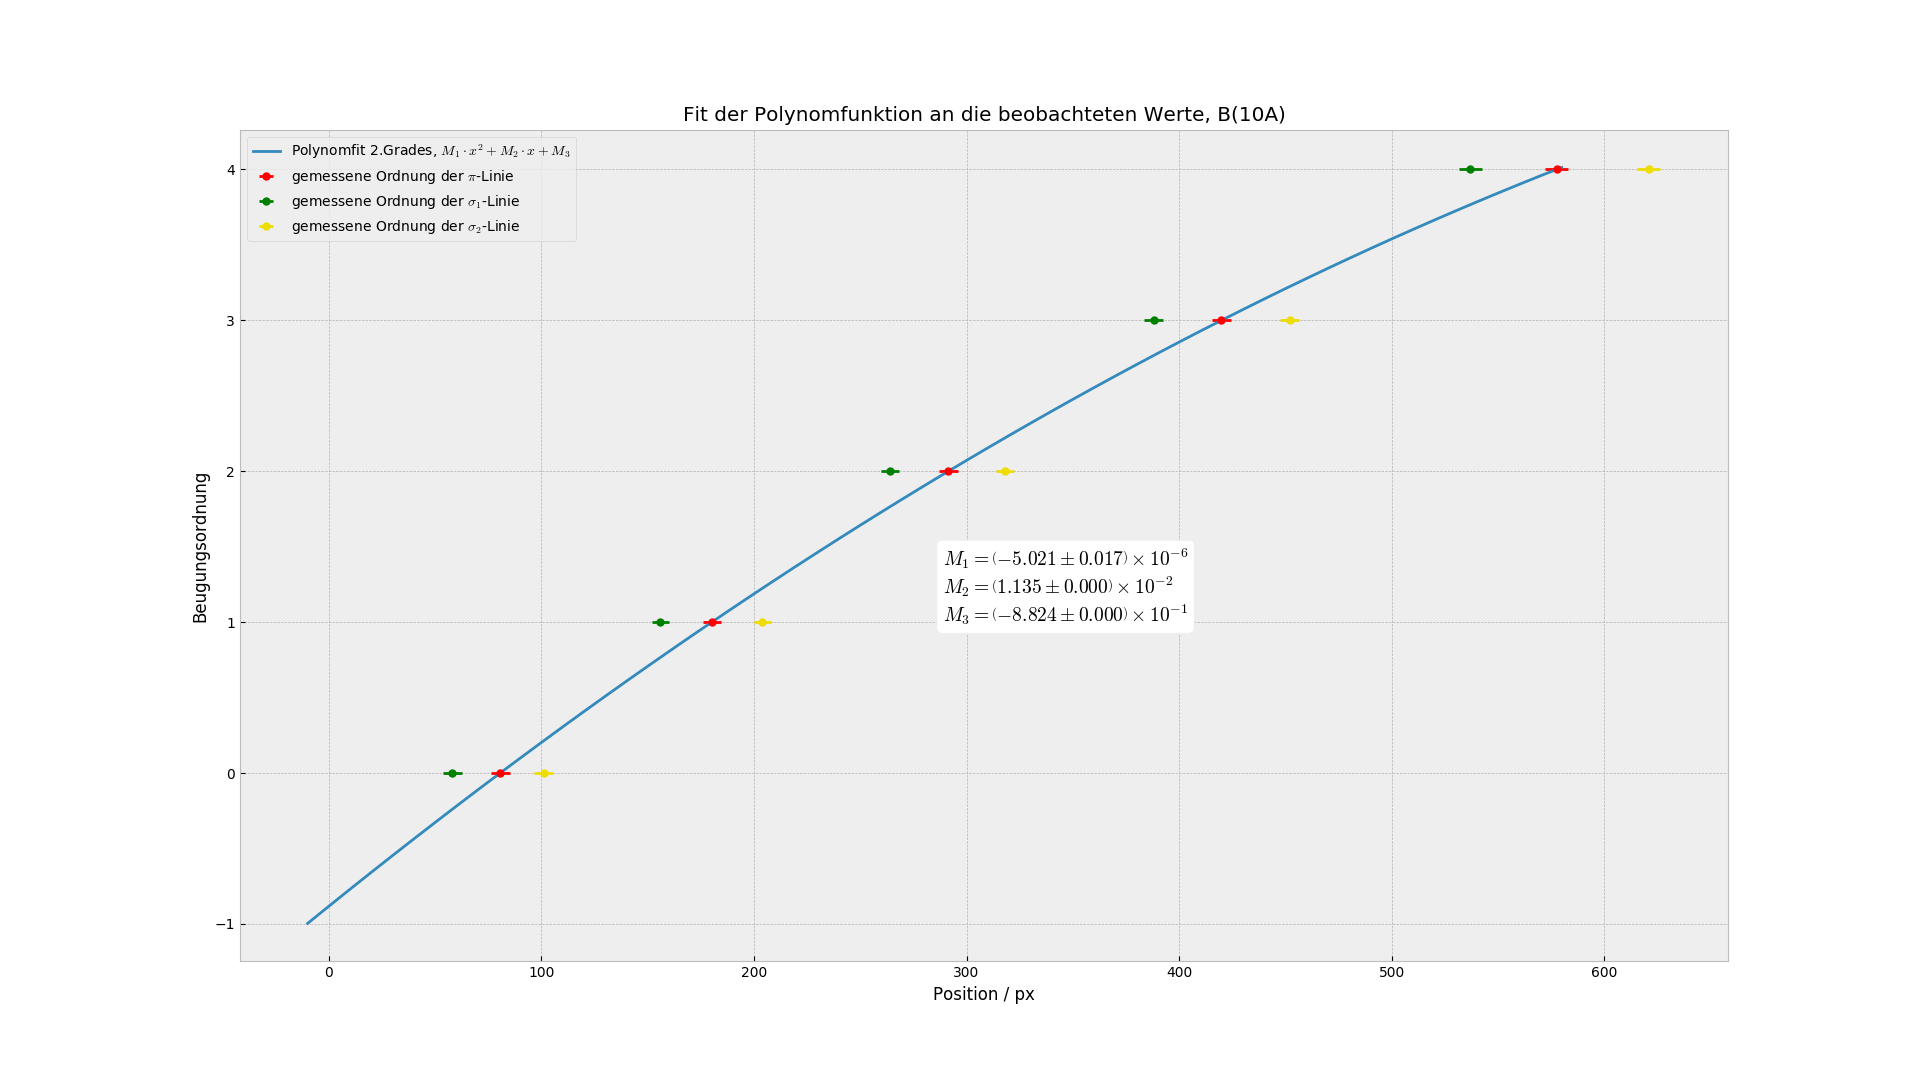
\includegraphics[width=.45\paperwidth]{Auswertung/scatterorder/sco_10A}
            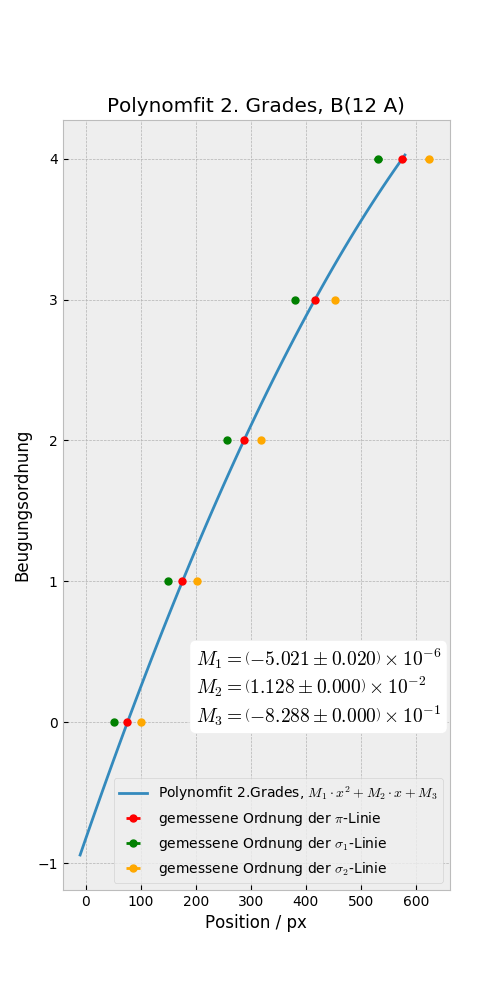
\includegraphics[width=.45\paperwidth]{Auswertung/scatterorder/sco_12A}
            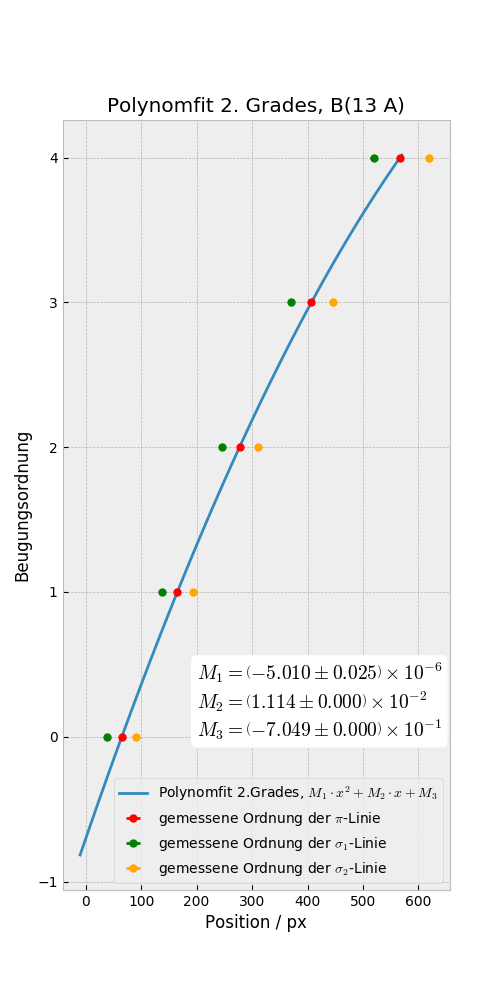
\includegraphics[width=.45\paperwidth]{Auswertung/scatterorder/sco_13A}
          \end{figure}
        \end{landscape}
        \begin{landscape}
          \thispagestyle{empty}
          \begin{figure}
            \vspace*{-2cm}
            \caption{Verschiebung der Beugungsordnung}
            \label{plot::3.5}
            \hspace*{-5cm}\vspace{-1cm}
            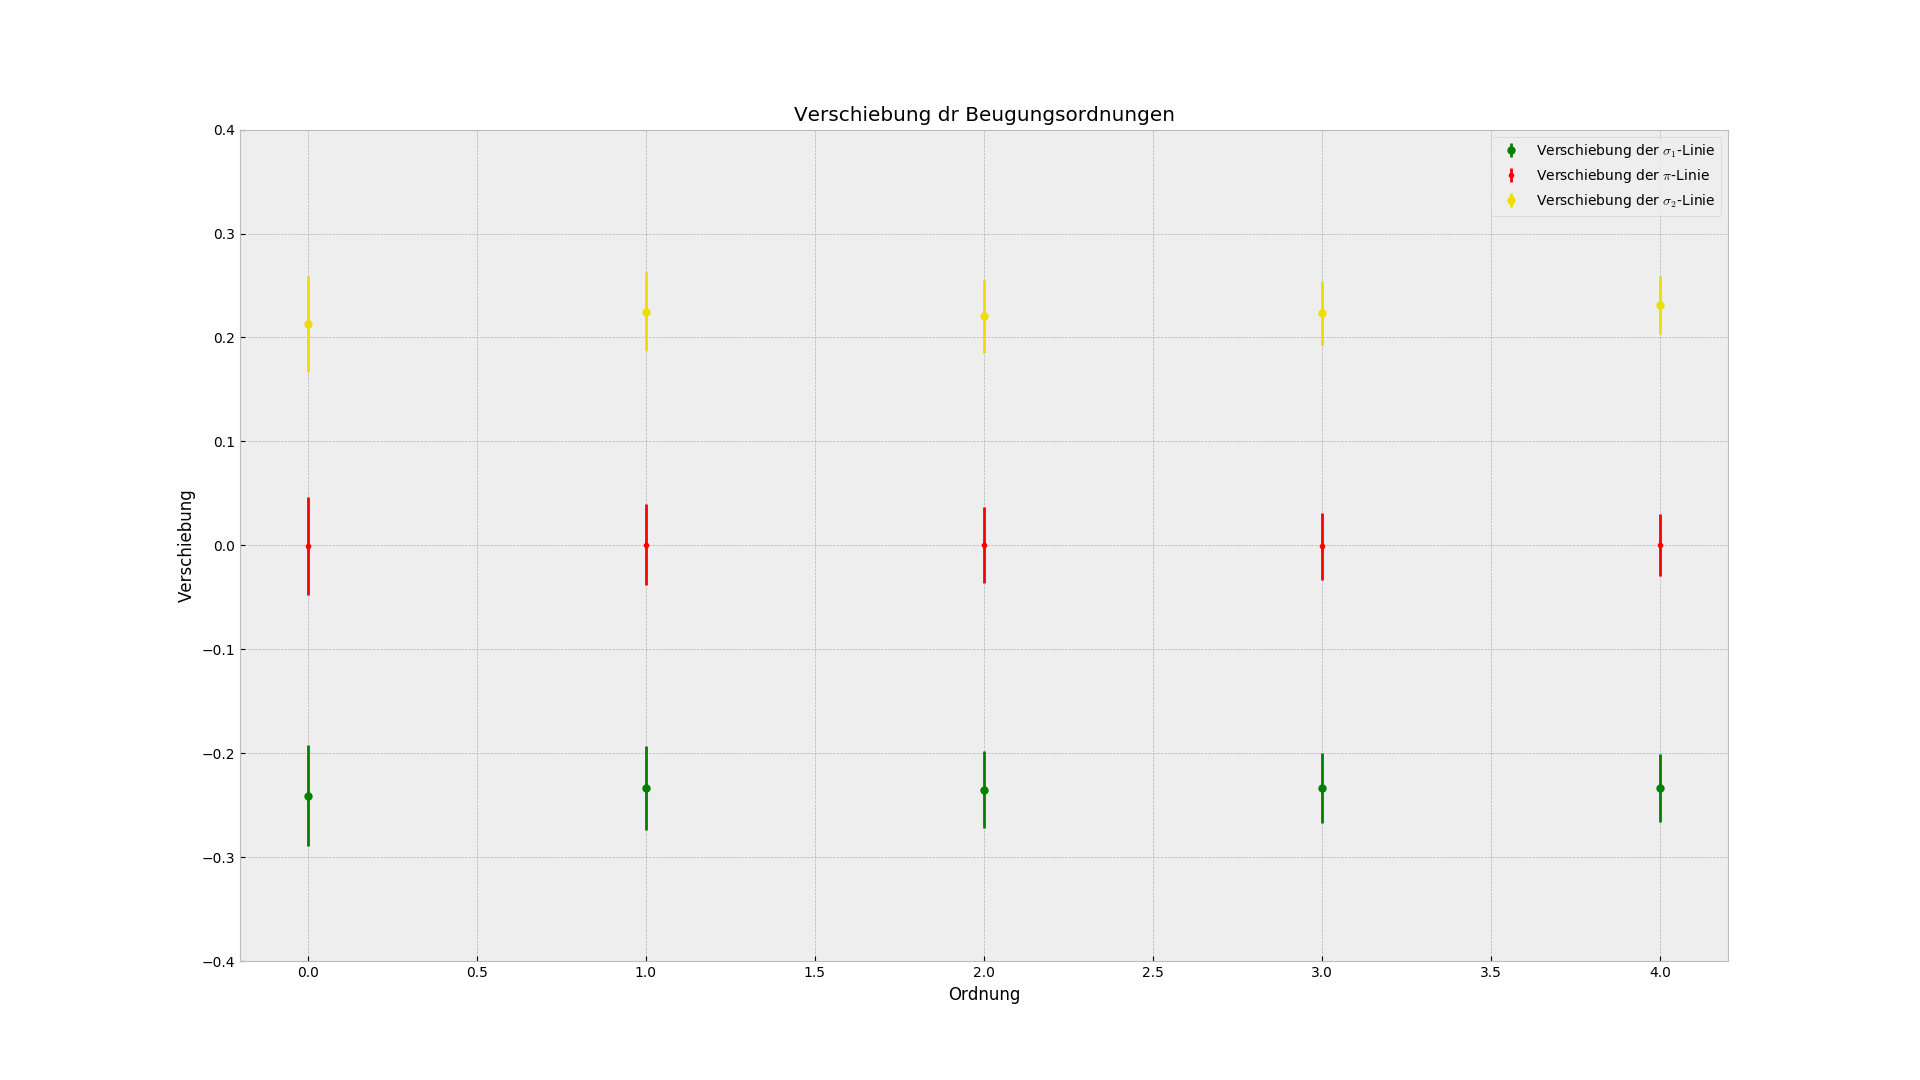
\includegraphics[width=.45\paperwidth]{Auswertung/scatterorder/diff_sco10A}
            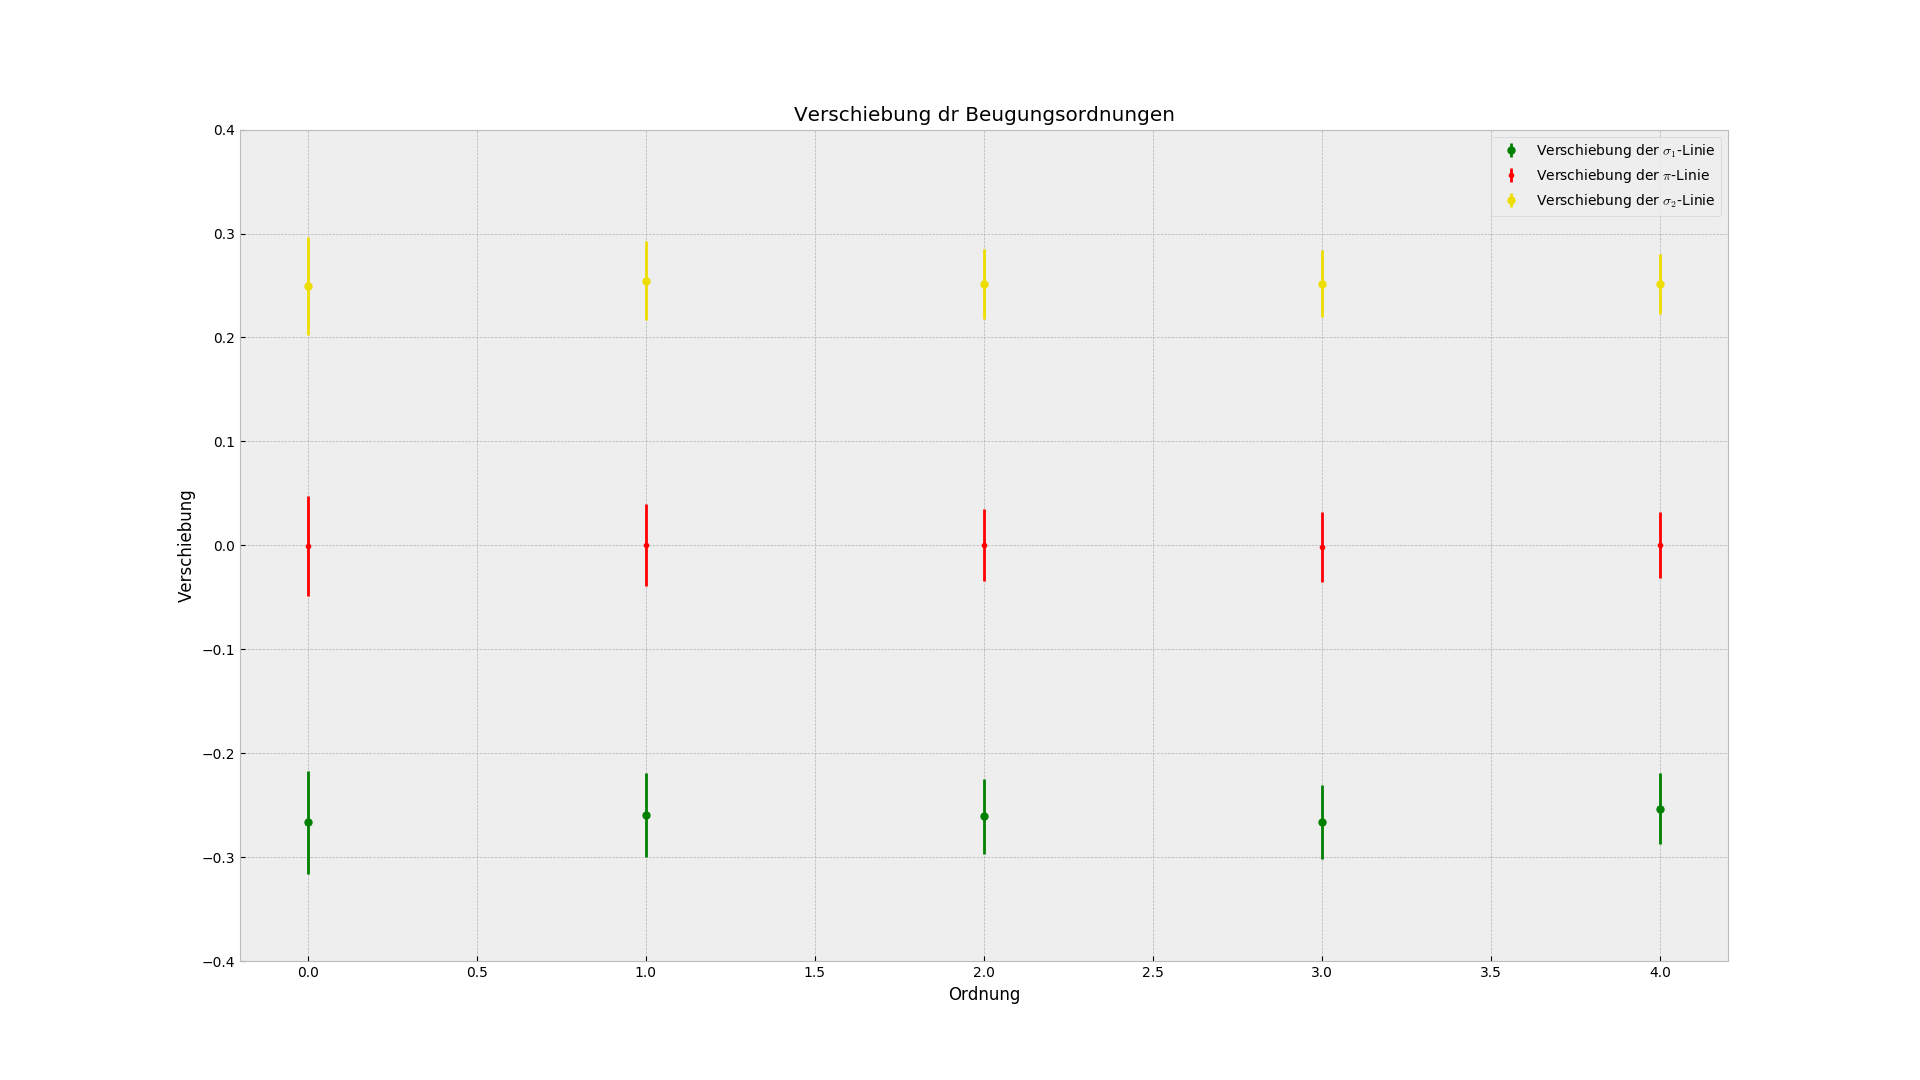
\includegraphics[width=.45\paperwidth]{Auswertung/scatterorder/diff_sco12A}
            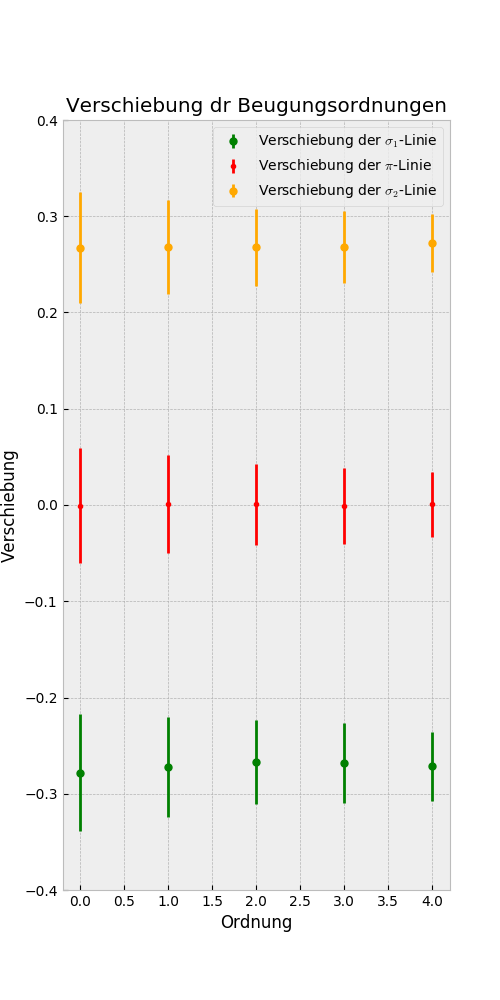
\includegraphics[width=.45\paperwidth]{Auswertung/scatterorder/diff_sco13A}
          \end{figure}
        \end{landscape}

      \subsubsection{Wellenlängenverschiebung}
        Um die Verschiebung der Wellenlänge zu erhalten nutzen wir die errechneten Werte in Bruchteilen der Beugungsordnung.
        \begin{align}
          \delta \lambda = \frac{\delta a}{\Delta a}\cdot \Delta \lambda \approx \delta k\cdot \Delta\lambda \label{fml::2}
        \end{align}
        Wobei die benutzte Näherung nur für kleine Verschiebungen gilt, in der der betrachtete Bereich der quadratischen Funktion als linear angesehen werden kann. Mithilfe von \hyperref[fml::1]{Gl. (\ref*{fml::1})}
        und \hyperref[fml::2]{Gl. (\ref*{fml::2})} kann jetzt die Wellenlängenverschiebung berechnet werden. Für die Wellenlänge $\lambda_{Cd}$ der roten Cadmium-Linie sowie deren Fehler verwenden wir den in Teil 2 ermittelten Wert \hyperref[val::lcd]{Gl. (\ref*{val::lcd})}:
        \begin{align}
          \lambda_{Cd} = \SI{643.927+-0.571}{\nano\metre}
        \end{align}
        ($n = \SI{1.4567}{}, d=\SI{4.04e-3}{m}$)

        Aus den Ergebnissen der untersuchten Ordnungen (\hyperref[plot::3.5]{Abb. \ref*{plot::3.5}}) lässt sich ein Mittelwert mit statistischem Fehler berechnen, um so jeweils einen Wert für die Wellenlängenverschiebung der beiden σ-Linien zu erhalten. Da das Experiment bei drei verschiedenen Magnetfeldern durchgeführt wurde, ergeben sich so sechs Werte, die nachfolgend in einer Tabelle zusammengefasst sind.
        \begin{table}[H]
          \centering
          \begin{tabular}{lll}
\toprule
I/A & $\delta\lambda_1/\si{pm}$ & $\delta\lambda_2/\si{pm}$ \\
\midrule
 10 &       $-11.394 \pm 0.140$ &        $10.788 \pm 0.294$ \\
 12 &       $-12.656 \pm 0.239$ &        $12.197 \pm 0.087$ \\
 13 &       $-13.153 \pm 0.187$ &        $13.019 \pm 0.093$ \\
\bottomrule
\end{tabular}

          \caption{Wellenlängenverschiebung für die drei beobachteten Stromstärken, sowie für beide $\sigma$-Linien}
          \label{tab::1}
        \end{table}

      \subsection{Bestimmung des Bohr'schen Magnetons}
        Das äußere Magnetfeld verursacht eine Verschiebung des Energieniveaus in Cadmium, diese Differenz lässt sich mit Hilfe der zuvor bestimmten Wellenlängenverschiebung der Spektrallinien berechnen:
        \begin{align}
          \Delta E         &= \frac{hc}\lambda-\frac{hc}{\lambda+\delta\lambda}\\
          \Delta(\Delta E) &= \frac{hc}{(\lambda+\delta\lambda)^2}\cdot\Delta(\delta\lambda)
        \end{align}
        Zwischen angelegtem Magnetfeld und der Energieverschiebung gilt \hyperref[fml::3]{Gl. (\ref*{fml::3})}

        Wir bestimmen das Magneton nun auf zwei unterschiedliche Arten:

        \subsubsection{Methode 1 - statistisches Mittel}
          Wir kennen jetzt die Werte des Magnetfeldes, sowie die entsprechende Energieverschiebung und können nun das Magneton berechnen:
          \begin{align}
            \mu_B=\left| \frac{\Delta E}{B} \right|
          \end{align}
          Wir erhalten erneut sechs Werte, sowie deren Fehler:
          \begin{table}[H]
            \centering
            \begin{tabular}{lll}
\toprule
I/A & $\mu_{B1}/(10^{-24}\si{\joule\per\tesla})$ & $\mu_{B2}/(10^{-24}\si{\joule\per\tesla})$ \\
\midrule
 10 &                         $10.446 \pm 0.461$ &                          $9.890 \pm 0.499$ \\
 12 &                         $10.090 \pm 0.452$ &                          $9.724 \pm 0.401$ \\
 13 &                          $9.845 \pm 0.418$ &                          $9.744 \pm 0.396$ \\
\bottomrule
\end{tabular}

            \caption{Bohr'sches Magneton, nach Methode 1, für beide $\sigma$-Linien}
            \label{tab::2}
          \end{table}~\\
          Der gesamte Mittelwert aus diesen Daten ist dann:

          \begin{align}
            \mu_B         &= \magnetonOne\\
            \mu_{B, theo} &= \magnetonTheo %TODO insert source
          \end{align}
          Der hier ermittelte Wert und der gegebene Theoriewert stimmen dabei innerhalb von \SI{1.6}{\sigma} überein.

        \subsubsection{Methode 2 - linearer Fit}
        Der lineare Zusammenhang, zwischen Magnetfeld und Energieverschiebung, lässt auch eine graphische Bestimmung des Bohr'schen Magnetons zu. Hier wird die Energieverschiebung gegen das Magnetfeld aufgetragen und linear gefittet. Die Steigung dieses Fits entspricht dem Wert für das Bohr'sche Magneton. Der Mittelwert beider Werte gibt das Endergebnis an.

        \begin{align}
          \mu_B = \magnetonTwo
        \end{align}
        Allerdings liegt hier die Abweichung zum Literaturwert bei \SI{4.2}{\sigma}, und ist somit signifikant.
        \begin{figure}[H]
          \centering
          \hspace*{-1.5cm}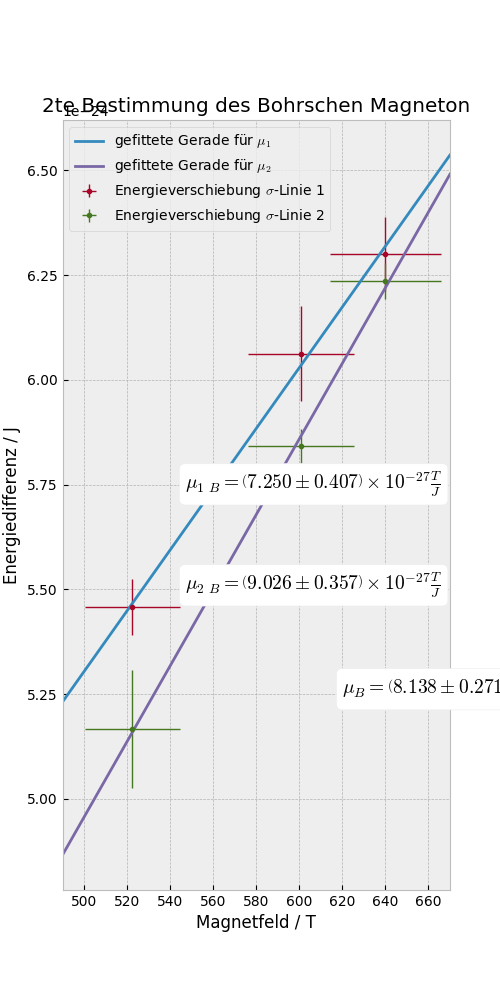
\includegraphics[width=1.2\textwidth]{Auswertung/mu_B2}
          \caption{Graphische Bestimmung des Bohr'schen Magneton}
          \label{plot::4}
        \end{figure}

  \section{Teil 2: Wellenlänge}
  In diesem Versuchsteil gilt es die genaue Wellenlänge der Cadmium-Linie zu bestimmen, Wir nutzen dazu zunächst das Spektrum einer Neon-Lampe als Referenz.
  Wir bestimmen wie zuvor mit \textbf{JImage} und \textbf{Python} die Position der Linien mit Hilfe eines Gauss-Fits.

  Das aufgenommene Spektrum sowohl der Neon-, als auch der Cadmium-Lampe sind in \hyperref[plt::5]{Abb. \ref*{plt::5}} zu sehen, für welches die folgenden Referenzwerte genutzt werden:
  \begin{align}
    \lambda_{Ne,1} = \SI{633.443}{\nano\metre}\nonumber\\
    \lambda_{Ne,2} = \SI{638.299}{\nano\metre}\nonumber\\
    \lambda_{Ne,3} = \SI{640.225}{\nano\metre}\nonumber\\
    \lambda_{Ne,4} = \SI{650.623}{\nano\metre}\nonumber\\
    \lambda_{Ne,5} = \SI{653.288}{\nano\metre}\nonumber\\
    \lambda_{Ne,6} = \SI{659.895}{\nano\metre}
  \end{align}


  \begin{figure}[H]
    \centering
    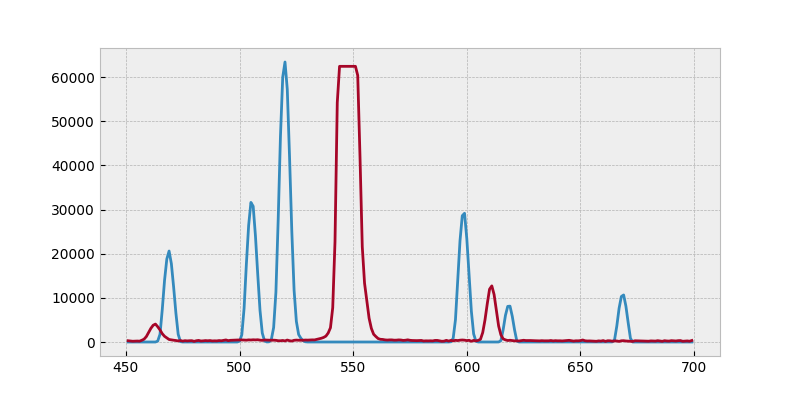
\includegraphics[width=\textwidth]{Auswertung/wavelength_analysis/wl}
    \caption{Cadmium- (Rot) und Neon- (Blau) Linien, y-Achse arbiträr}
    \label{plt::5}
  \end{figure}

  \subsection{Cadmium-Linie}
    Aus den so bestimmten Werten ergibt sich der folgende Zusammenhang (\hyperref[plt::6]{Abb. \ref*{plt::6}}), für Position und Wellenlänge, sowie die Wellenlänge der Cadmium-Linie.
    \begin{align}
      a_{Cd}       &= \SI{547.945+-4.310}{px}\\
      \lambda_{Cd} &= \lambdaCd \label{val::lcd}
      \intertext{mit dem Theoriewert}
      \lambda_{Cd,theo} &= \lambdaCdTheo
    \end{align}
    und einer Abweichung von \SI{.14}{\sigma}

    \subsection{unbekannte Linie}
      In unserem Spektrum sollte sich eine weitere Linie befinden, welche bei etwa $\SI{652}{\nano\metre}$ zu erkennen sei. diese liegt bei uns bei
      \begin{align}
        \lambda_{uk} = \lambdaUk
      \end{align}
      was nach \cite{nist.gov.uk}, entweder mit Thorium oder Xenon übereinstimmt
      \begin{align}
        \lambda_{Th I, L5951} = \lambdaTh\\
        \lambda_{Xe I, L7292} = \lambdaXe
      \end{align}
      Wir nehmen an, dass es sich hierbei um Xenon handelt, da dieses gasförmig und nichtmetallisch ist.

    \begin{landscape}
      \thispagestyle{empty}
      \begin{figure}
        \vspace*{-2cm}
        \caption{Zusammenhang zwischen Position und Wellenlänge in unseren Beobachtungen}
        \hspace*{-6cm}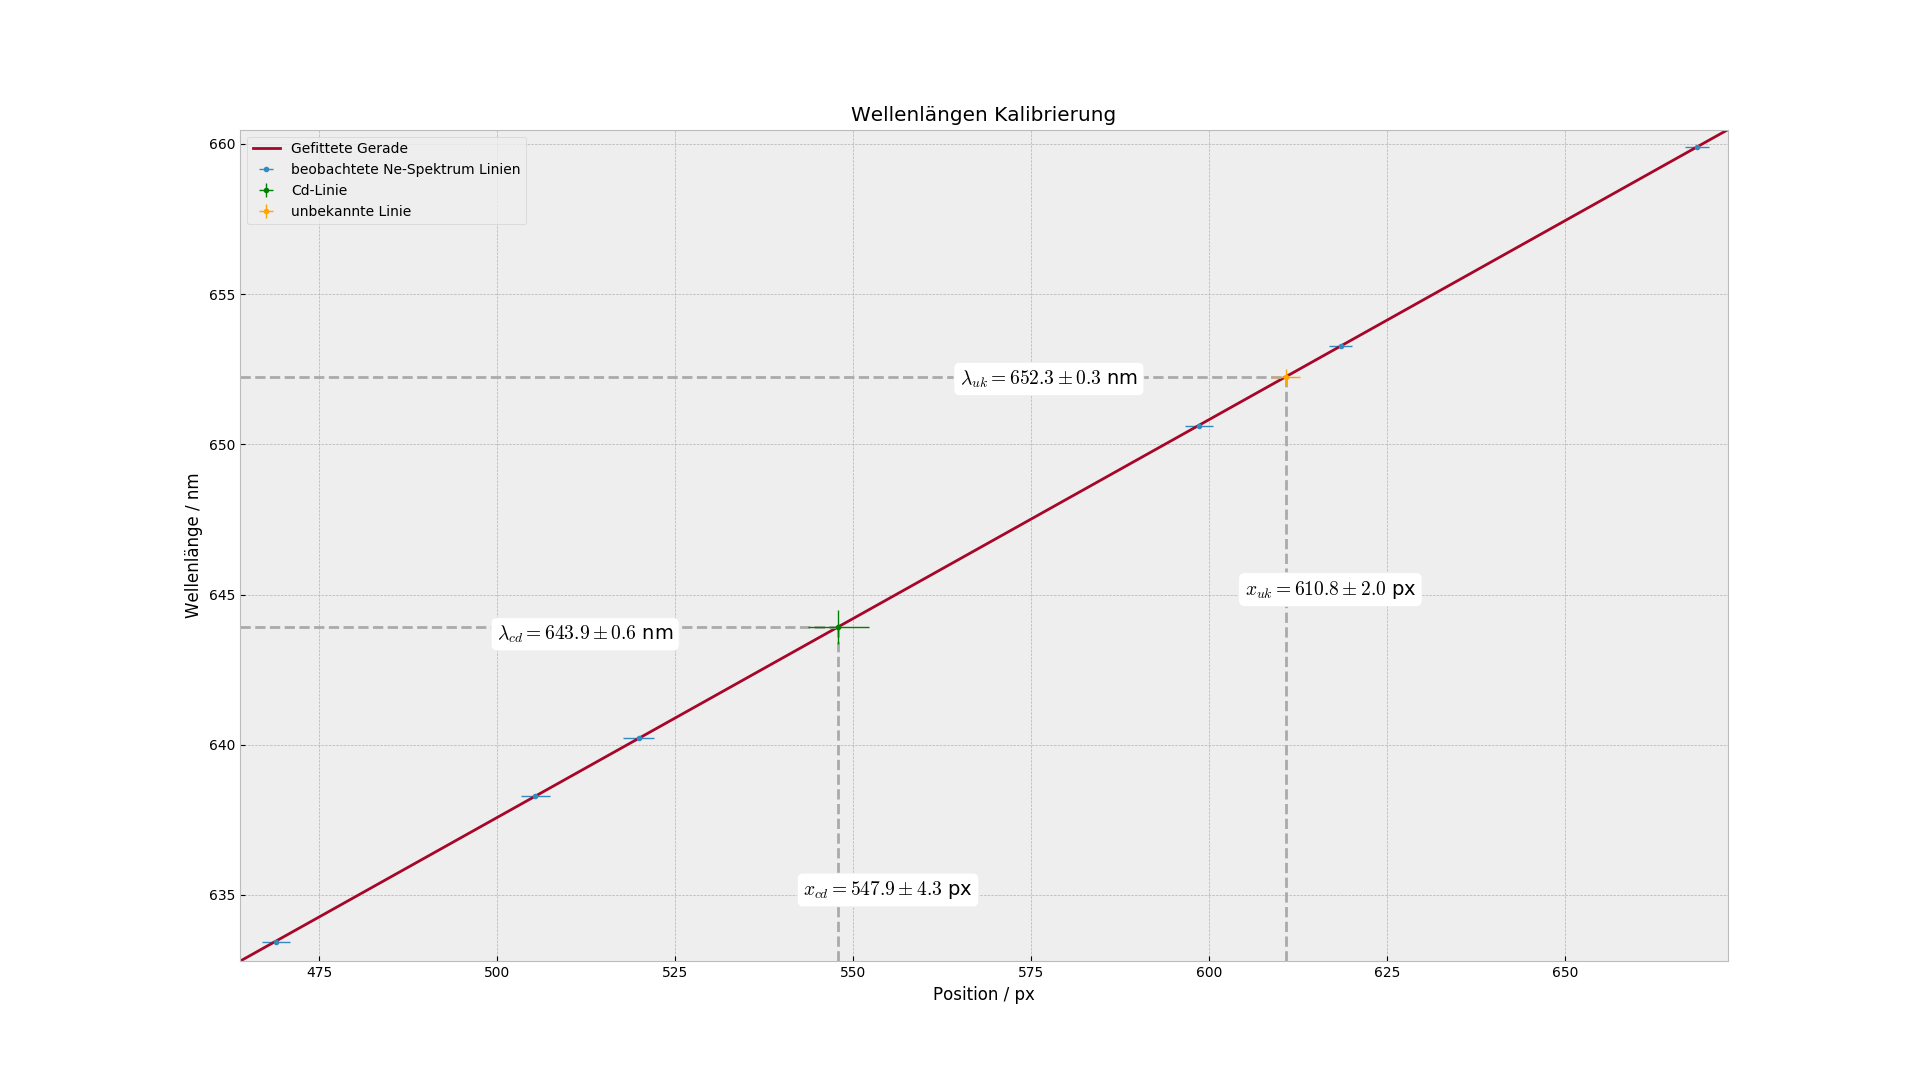
\includegraphics[width=1.5\paperwidth]{Auswertung/wavelength_analysis/wl_ne_cal}
        \label{plt::6}
      \end{figure}
    \end{landscape}

  \section{Diskussion und Zusammenfassung}
  Der erste Teil des Versuchs bestand darin, zuerst herrauszufinden ob in unseren Beobachtungen der Hysterese Effekt zu berücksichtigen war und der Erhalt des Verhältnisses zwischen elektrischem Strom und Magnetfeldstärke.
  Bei uns war der Hysterese-Effekt zu vernachlässigen.

  Weiterhin wurden qualitative Aussagen über die Polarisation der Übergänge in Cadmium untersucht, welche mit den gemachten Beobachtungen übereinstimmen.

  Danach konnten die beobachteten Spektallinien einer Cd-Lampe mit Hilfe einer Lummer-Gehrcke Platte und einer CCD Kamera untersucht werden, welche uns aus der Beobachtung des Interferenzmusters von $\pi$- und $\sigma$-Linien einen Wert für das Bohr'sche Magneton, auf zwei Arten lieferte. Beide Methoden ergaben dabei unterschiedliche Ergebnisse, wobei das mit Hilfe des arithmetischen Mittels berechnete Erbegnis genauer mit dem Literaturwert überein stimmt. Mathematisch sollten bei beiden Methoden die selben Werte gefunden werden.
  \begin{align*}
    \mu_{B,1} &= \magnetonOne\\
    \mu_{B,2} &= \magnetonTwo\\
    \mu_{B,Theo} & = \magnetonTheo
  \end{align*}
  Dabei sollte erwähnt werden, dass der lineare Fit einen eher größeren Fehler besitzt, da dieser nur zwischen drei Messpunkten stattfand und ausserdem kein lineares Verhalten aufweist, das kann daran liegen, dass das Magnetfeld im Bereich zwischen 12 und 13A bereits in Sättigung geht und somit unser Zusammenhang zwischen Strom und Magnetfeld nicht mehr als linear angenommen werden sollte. Was ausserdem in einer geringeren Aufspaltung der Linien resultiert.
  Man könnte diesen Effekt vermeiden, indem man kleinere Änderungen des Stroms betrachtet.

  Im Zweiten Teil des Versuchs, galt es Wellenlängen den Linien des Cadmium-Spektrums zuzuordnen. Dabei fanden wir für die Hauptlinie eine sehr gute Übereinstimmung mit dem Literaturwert
  \begin{align*}
    \begin{rcases}
      \lambda_{Cd} &=\lambdaCd \quad\\
      \lambda_{Cd, Theo} &= \lambdaCdTheo
    \end{rcases}
    \quad\text{Abw.: }\SI{.14}{\sigma}
  \end{align*}

  Zudem sollte eine Wellenlänge einer unbekannten Linie zugeordnet werden, diese stimmt unserer Meinung nach mit einer Linie des Xe(I)-Spektrums überein

  \begin{align*}
    \begin{rcases}
      \lambda_{uk} &= \lambdaUk\quad\\
      \lambda_{Xe I, } &= \lambdaXe
    \end{rcases}
    \quad\text{Abw.: }\SI{.38}{\sigma}
  \end{align*}

  \begin{thebibliography}{9}

\bibitem{czerny.turner}
  \href{https://de.wikipedia.org/wiki/Monochromator#/media/File:Czerny-turner.png}{Czerny-Turner Spektrometer},
  Wikipedia,
  10.09.17

\bibitem{fp.booklet}
  \href{http://www.physi.uni-heidelberg.de/Einrichtungen/FP/anleitungen/F44.pdf}{Literaturwert des Bohrschen Magnetons},
  F44 Versuchsanleitung von FP-Server,
  20.06.17

\bibitem{nist.gov.cd}
  \href{https://physics.nist.gov/PhysRefData/Handbook/Tables/cadmiumtable2.htm}{Literaturwerte des Cadmium Spektrums},
  NIST,
  01.09.17

\end{thebibliography}

\end{document}
